%%%%%%%%%%%%%%%%%%%%%%%%%%%%%%%%%%%%%%%%%%%%%%%%%%%%%%%%%%%%%%%%%%%%%%%%%%%%%%%
% Author:  Pablo Alvarado
%
% Escuela de Ingeniería Electrónica
% Instituto Tecnológico de Costa Rica
%
% Tesis de Licenciatura
% 
% Phone:   +506 2550 9005
% email:   palvarado@itcr.ac.cr
%
%%%%%%%%%%%%%%%%%%%%%%%%%%%%%%%%%%%%%%%%%%%%%%%%%%%%%%%%%%%%%%%%%%%%%%%%%%%%%%%

% \documentclass is book
% If you want a printable two-side version of the thesis
%\documentclass[12pt,twoside,letterpaper]{book}

% If you want an electronic-only version of the thesis, do it one-sided
\documentclass[12pt,oneside,letterpaper]{book}

\usepackage[T1]{fontenc}
%\usepackage[utf8]{inputenc}   % is no longer required (since 2018)
\usepackage{ifthen}            % provide if-then-else operators

% --------------------------------------------------------------------------
% Global variables required in document formatting
% --------------------------------------------------------------------------
%
% BOOK MODE
%
\newboolean{bookmode}                  % boolean used to control book format
% Ensure that only one of the next two lines is active:
\setboolean{bookmode}{true}           % turn book mode on
%\setboolean{bookmode}{false}           % turn book mode off

%
% DRAFT MODE
%   The draft mode activates the TODO index and some "draft" markings all
%   around.  Ensure you set it to false for the final version!!
%   
%
\newboolean{draftmode}                  % boolean used to control draft-mode

%% -------------------------------------------------------------------------

%% Configure su nombre, título de tesis, lectores, fechas, etc. en:
%%
%% >>>>  config.tex  <<<<
%%

% --------------------------------------------------------------------------

% include all packages and define all required general macros
%%%%%%%%%%%%%%%%%%%%%%%%%%%%%%%%%%%%%%%%%%%%%%%%%%%%%%%%%%%%%%%%%%%%%%%%%%%%%%%
% Author:  Pablo Alvarado
%
% Escuela de Electrónica
% Instituto Tecnológico de Costa Rica
%
% Phone:   +506 2550 9005
% email:   palvarado@itcr.ac.cr
% 
%%%%%%%%%%%%%%%%%%%%%%%%%%%%%%%%%%%%%%%%%%%%%%%%%%%%%%%%%%%%%%%%%%%%%%%%%%%%%%%

\PassOptionsToPackage{usenames,dvipsnames,table}{xcolor}

% -----------------------------------------------------------------------------
%   Define all configuration commands
% -----------------------------------------------------------------------------

\newcommand{\genderLector}[1]{%
  \ifthenelse{\equal{#1}{F}}{%
    Profesora Lectora%
  }{%
    \ifthenelse{\equal{#1}{M}}{%
      Profesor Lector%
    }{%
      Persona profesora lectora%
    }%
  }%
}

% Lector I
\newcommand{\nameLectorI}{$<$\emph{Use defLectorI in config.tex}$>$}
\newcommand{\genderLectorI}{N/A}

\newcommand{\defLectorI}[1][M]{%
  \renewcommand{\genderLectorI}{\genderLector{#1}}%
  \lectorIRelay%
}

\newcommand{\lectorIRelay}[1]{%
  \renewcommand{\nameLectorI}{#1}
}

%% Lector II
\newcommand{\nameLectorII}{$<$\emph{Use setLectorII in main.tex}$>$}
\newcommand{\genderLectorII}{N/A}

\newcommand{\defLectorII}[1][M]{%
  \renewcommand{\genderLectorII}{\genderLector{#1}}%
  \lectorIIRelay%
}

\newcommand{\lectorIIRelay}[1]{%
  \renewcommand{\nameLectorII}{#1}
}

%% Asesor
\newcommand{\nameAsesor}{$<$\emph{Use setAsesor in main.tex}$>$}
\newcommand{\genderAsesor}{$<$\emph{Use setAsesor in main.tex}$>$}

\newcommand{\defAsesor}[1][M]{%
  \ifthenelse{\equal{#1}{F}}{%
    \renewcommand{\genderAsesor}{Profesora Asesora}%
  }{%
    \ifthenelse{\equal{#1}{M}}{%
      \renewcommand{\genderAsesor}{Profesor Asesor}%
    }{%
      % La RAE no ha definido cómo hacer esto...
      %
      % Hay que preguntar a la persona asesora no-binaria directamente
      % cómo gusta ser tratada.
      \renewcommand{\genderAsesor}{Persona profesora asesora}%
    }
  }
  \asesorRelay
}

\newcommand{\asesorRelay}[1]{%
  \renewcommand{\nameAsesor}{#1}
}

% Dates for draft and final
\newcommand{\thesisDraftDate}{\today}
\newcommand{\defDraftDate}[1]{\renewcommand{\thesisDraftDate}{#1}}

\newcommand{\thesisFinalDate}{$<$\emph{Fecha de Defensa en config.tex}$>$}
\newcommand{\defFinalDate}[1]{\renewcommand{\thesisFinalDate}{#1}}

% Author definition and gender related strings

\newcommand{\thesisAuthor}{Error: Undefined}
\newcommand{\thesisAuthorShort}{Error: Undefined}
\newcommand{\thesisAuthorTECID}{Error: Undefined}
\newcommand{\thesisAuthorAddress}{Error: Undefined}
\newcommand{\thesisAuthorDegree}{Error: Undefined}

\newcommand{\defAuthor}[1][M]{%
  \ifthenelse{\equal{#1}{F}}{%
    \renewcommand{\thesisAuthorAddress}{la señora}
    \renewcommand{\thesisAuthorDegree}{Ingeniera}
  }{%
    \ifthenelse{\equal{#1}{f}}{%
      \renewcommand{\thesisAuthorAddress}{la señorita}
      \renewcommand{\thesisAuthorDegree}{Ingeniera}
    }{%
      \ifthenelse{\equal{#1}{M}}{%
        \renewcommand{\thesisAuthorAddress}{el señor}
        \renewcommand{\thesisAuthorDegree}{Ingeniero}
        
      }{%
        \renewcommand{\thesisAuthorAddress}{la persona}
        \renewcommand{\thesisAuthorDegree}{Ingeniere}
      }
    }
  }
  \authorRelay
}

\newcommand{\authorRelay}[1]{%
  \renewcommand{\thesisAuthor}{#1}
}

\newcommand{\defAuthorShort}[1]{%
  \renewcommand{\thesisAuthorShort}{#1}
}

\newcommand{\defAuthorTECID}[1]{%
  \renewcommand{\thesisAuthorTECID}{#1}
}

%% About the institution and department
\newcommand{\thesisDepartment}{Escuela de Ingeniería Electrónica}
\newcommand{\thesisInstitution}{Tecnológico de Costa Rica}

\newcommand{\defDepartment}[1]{%
  \renewcommand{\thesisDepartment}{#1}
}

\newcommand{\defInstitution}[1]{%
  \renewcommand{\thesisInstitution}{#1}
}



%% About the report name, and type
\newcommand{\thesisTitle}{Error: Undefined}
\newcommand{\thesisFlatTitle}{\thesisTitle}
\newcommand{\thesisKeywords}{Error: Undefined}
\newcommand{\thesisType}{Error: Undefined}

%% A tool to remove new lines leaving no spaces
\newcommand\titleFlattener[1]{\def\\{\relax\ifhmode\unskip\fi\space\ignorespaces}#1}

\newcommand{\defTitle}[1]{%
  \renewcommand{\thesisFlatTitle}{\titleFlattener{#1}}
  \renewcommand{\thesisTitle}{#1}
}

\newcommand{\defKeywords}[1]{%
  \renewcommand{\thesisKeywords}{#1}
}

\newcommand{\defTFGType}[1]{%
  \renewcommand{\thesisType}{#1}
}

%% Este archivo contiene toda la configuración básica del documento de
%% tesis, para centralizar alguna información que se requiere en todo
%% el documento.

%% DRAFT MODE

%%   El modo borrador activa las listas de cosas por hacer, con su
%%   índice, y algunas marcas explícitas de "borrador" por todo lado.
%%
%%   Asegúrse de que esta variable sea false en la versión final y de haber
%%   actualizado la fecha de la defensa, un poco más abajo.
\setboolean{draftmode}{true}            % turn draft mode on
%\setboolean{draftmode}{false}          % turn draft mode off

%% Esta es la fecha que se colocará en el modo borrador
\defDraftDate{\today}
%% Esta es la fecha que se usará en la versión final
\defFinalDate{24 de noviembre, 2023}

%% Este es el nombre del estudiante y el pronombre que utiliza, para cambiar
%% las portadas como corresponde

% Con el nombre de autor, se debe especificar el género a utilizar:
%
%   [M]asculino
%   [F]emenino (usando "señora" donde corresponda)
%   [f]emenino (usando "señorita" donde corresponda)
%   persona [N]o binaria
%
%   Debido a la falta de norma en español para las personas no binarias,
%   posíblemente deba ajustarse para el gusto de cada quien.
%
\defAuthor[M]{Oscar Andrés Rojas Fonseca}                % Nombre del estudiante
%\defAuthor[f]{María del Pilar Pérez Prado}    % Nombre de la estudiante

\defAuthorShort{O.~Rojas}                      % Nombre corto
\defAuthorTECID{2018102187}                     % Carné

%% Este es el título completo del informe del trabajo final de graduación.
%% Usted puede agregar \\ para forzar líneas nuevas en la portada y automática-
%% mente el comando se encarga de eliminar eso cuando necesita el título
\defTitle{Método basado en aprendizaje reforzado \\% 
para el control automático de una \\%
planta no lineal}

%% Palabras clave
\defKeywords{palabras, clave, energía, cambio climático, RISC V}

%% Tribunal Evaluador
%%
%% Indique los nombres de los lectores y asesor
%% El parámetro opcional es
%%  [M]asculino,
%%  [F]emenino,
%%  persona [N]o binaria
\defLectorI[F]{Dra.\,María Curie Pérez}
\defLectorII[M]{M.Sc.\,Pedro Pérez Pereira}
\defAsesor[M]{Ing.\,Albert Einstein Sánchez}

%% Tipo de tesis o informe
%%   - Tesis de Licenciatura
%%   - Informe de Proyecto Final 
%%   - Tesis de Maestría
\defTFGType{Tesis de Licenciatura}

%% Nombre del departamento e institución
\defInstitution{Instituto Tecnológico de Costa Rica}
\defDepartment{Escuela de Ingeniería Electrónica}

 % Load the desired configuration

%Para el PDF (cambiar si se desea otras cosas a lo indicado arriba
\newcommand{\pdfAuthor}{\thesisAuthor}
\newcommand{\pdfTitle}{\thesisFlatTitle} 
\newcommand{\pdfKeywords}{\thesisKeywords}
\newcommand{\pdfSubject}{\thesisType}


%% -------------------------------------------------------------------

\usepackage{ifpdf}

% Command to change between draft or release mode:
\newcommand{\ifdraft}[2]{\ifthenelse{\boolean{draftmode}}{#1}{#2}}
% Command to change between draft or release mode:
\newcommand{\ifbook}[2]{\ifthenelse{\boolean{bookmode}}{#1}{#2}}

% include all required packages here
\usepackage{csquotes}                  % recommended for biblatex
\usepackage[spanish,es-tabla]{babel}   % spanish, remove es-tabla for cuadro
%\usepackage[spanish]{babel}   % spanish, remove es-tabla for cuadro

\usepackage{xspace} % Decide if a space is needed at the end of some commands

\makeatletter
% babel uses a hook and therefore the tablename is here not defined yet.
% However, it defines es@tablename with upper/lowercase, and we use it.
\ifthenelse{\equal{\es@tablename}{Ttabla}}{%
  \newcommand{\cuadro}{tabla}
  \newcommand{\cuadros}{tablas}
  \newcommand{\Cuadro}{Tabla}
  \newcommand{\elcuadro}{la tabla}
  \newcommand{\Elcuadro}{La tabla}
  \newcommand{\loscuadros}{las tablas}
  \newcommand{\Loscuadros}{Las tablas}
  
  \newcommand{\tabla}{tabla}
  \newcommand{\tablas}{tablas}
  \newcommand{\Tabla}{Tabla}
  \newcommand{\latabla}{la tabla}
  \newcommand{\Latabla}{La tabla}
  \newcommand{\lastablas}{las tablas}
  \newcommand{\Lastablas}{Las tablas}
  
  \newcommand{\tabref}[1]{\hyperref[#1]{tabla~\ref*{#1}}\xspace}
  \newcommand{\Tabref}[1]{\hyperref[#1]{Tabla~\ref*{#1}}\xspace}

  \newcommand{\latabref}[1]{la \tabref{#1}}
  \newcommand{\Latabref}[1]{La \tabref{#1}}

}{%
  \newcommand{\cuadro}{cuadro}
  \newcommand{\cuadros}{cuadros}
  \newcommand{\Cuadro}{Cuadro}
  \newcommand{\elcuadro}{el cuadro}
  \newcommand{\Elcuadro}{El cuadro}
  \newcommand{\loscuadros}{los cuadros}
  \newcommand{\Loscuadros}{Los cuadros}
  
  \newcommand{\tabla}{cuadro}
  \newcommand{\tablas}{cuadros}
  \newcommand{\Tabla}{Cuadro}
  \newcommand{\latabla}{el cuadro}
  \newcommand{\Latabla}{El cuadro}
  \newcommand{\lastablas}{los cuadros}
  \newcommand{\Lastablas}{Los cuadros}
  
  \newcommand{\tabref}[1]{\hyperref[#1]{cuadro~\ref*{#1}}\xspace}
  \newcommand{\Tabref}[1]{\hyperref[#1]{Cuadro~\ref*{#1}}\xspace}

  \newcommand{\latabref}[1]{el \tabref{#1}}
  \newcommand{\Latabref}[1]{El \tabref{#1}}

}
\makeatother

% References to figures
\newcommand{\figref}[1]{\hyperref[#1]{figura~\ref*{#1}}\xspace}
\newcommand{\Figref}[1]{\hyperref[#1]{Figura~\ref*{#1}}\xspace}
\newcommand{\lafigref}[1]{la \hyperref[#1]{figura~\ref*{#1}}\xspace}
\newcommand{\Lafigref}[1]{La \hyperref[#1]{figura~\ref*{#1}}\xspace}

% References to equations
\newcommand{\equ}[1]{\hyperref[#1]{(\ref*{#1})}\xspace}

% Refrences to chapters and sections
\newcommand{\capref}[1]{\hyperref[#1]{capítulo~\ref{#1}}\xspace}
\newcommand{\secref}[1]{\hyperref[#1]{sección~\ref{#1}}\xspace}

\usepackage{makeidx}                    % to create index file

\usepackage[nottoc]{tocbibind}          % Fix the hyperrefs to TOC,TOF, etc.
                                        % and ensure that they appear all in 
                                        % the Table of Contents
\ifdraft{%
  %\usepackage[refpage]{nomencl}        % Use to easily administrate the list
  \usepackage[intoc,spanish]{nomencl}   % of symbols
}{%
  \usepackage[intoc,spanish]{nomencl}
}

\usepackage{siunitx}                    % Units of the SI
\sisetup{output-decimal-marker = {,}}   % Use decimal , instead of decimal .
\DeclareSIQualifier\peak{p}
\DeclareSIQualifier\ppeak{pp}

\usepackage{amsmath}
\usepackage{amssymb,amstext}            % AMS-math and symbols package
\usepackage{mathrsfs}                   % Calygraphic fonts for transforms
\usepackage{trsym}                      % Para símbolos de transformadas o---o
\usepackage{stmaryrd}                   % For short arrows
\usepackage{nicefrac}
\usepackage{array}                      % extensions to tabular environment
\usepackage{longtable}                  % supports extraordinary long tables
\usepackage{tabularx}                   % supports tables with fixed width

\usepackage[backend=biber,              % Use biber/biblatex
            style=ieee,
            sorting=none,
            citestyle=numeric-comp]{biblatex}

\usepackage{afterpage}                  % put something only after the page
\usepackage{multirow}                   % supports multiple row grouping in 
                                        % tables
\usepackage{multicol}                   % multiple columns environments
\usepackage{enumitem}                   % better enumeration with paralist 
                                        % equivalents as follows:

\newlist{compactitem}{itemize}{3}
\setlist[compactitem]{topsep=0pt,partopsep=0pt,itemsep=0pt,parsep=0pt}
\setlist[compactitem,1]{label=\textbullet}
\setlist[compactitem,2]{label=---}
\setlist[compactitem,3]{label=*}

\newlist{compactdesc}{description}{3}
\setlist[compactdesc]{topsep=0pt,partopsep=0pt,itemsep=0pt,parsep=0pt}

\newlist{compactenum}{enumerate}{3}
\setlist[compactenum]{label*=\arabic*.,topsep=0pt,partopsep=0pt,itemsep=0pt,parsep=0pt}
\newlist{compactenuma}{enumerate}{3}
\setlist[compactenuma]{label*=\alph*.,topsep=0pt,partopsep=0pt,itemsep=0pt,parsep=0pt}

\usepackage{icomma}                     % decimal comma in math mode

\usepackage{bold-extra}

\usepackage[format=hang,%
            font=small,%
            labelfont=bf]{caption}      % nicer figure captions
\usepackage{subcaption}                 % for subfigures
            
\usepackage{booktabs}                   % book type tabulars
\usepackage{pdfpages}                   % used to include the final "acta"

% the own style with options depending on the draft mode
\ifdraft{%
\usepackage[todo]{sty/tecStyle}         % some command definitions
                                        % options [todo] todo-index
}{%
\usepackage{sty/tecStyle}               % some command definitions
                                        % options [todo] todo-index
}

%% fix the title for examples
\renewcommand{\examplelistname}{Índice de ejemplos}
\renewcommand{\examplename}{Ejemplo}

%% define some command to cope with the tribunal names

%% Lector I


\usepackage{url}                        % allows linebreaks at certain
                                        % characters or combinations of 
                                        % characters for URLs

%% Usual tikz libraries and configuration
\usepackage{tikz}
\usepackage{pgfplots}
\pgfplotsset{compat=1.16}
\usepgfplotslibrary{fillbetween}
\usetikzlibrary{patterns,shapes,arrows.meta,positioning,calc,babel}
\usetikzlibrary{fit,shapes.geometric,decorations.markings}

\usepackage{listings}                   % syntax highlighting of code fragments

\lstdefinestyle{verilog-style}
{
  language=Verilog,
  basicstyle=\small\ttfamily,
  keywordstyle=\color{dkblue},
  identifierstyle=\color{black},
  commentstyle=\color{dkgreen},
  numbers=left,
  numberstyle=\tiny\color{black},
  numbersep=10pt,
  tabsize=8,
  moredelim=*[s][\colorIndex]{[}{]},
  literate=*{:}{:}1
}
\lstset{literate=%
  {á}{{\'a}}1
  {é}{{\'e}}1
  {í}{{\'i}}1
  {ó}{{\'o}}1
  {ú}{{\'u}}1
  {ñ}{{\~n}}1
  {Á}{{\'A}}1
  {É}{{\'E}}1
  {Í}{{\'I}}1
  {Ó}{{\'O}}1
  {Ú}{{\'U}}1
  {Ñ}{{\~N}}1
}

\definecolor{vorange}{RGB}{255,143,102}
\definecolor{tableheader}{rgb}{0.2,0.25,0.31}

\makeatletter
\newcommand*\@lbracket{[}
\newcommand*\@rbracket{]}
\newcommand*\@colon{:}
\newcommand*\colorIndex{%
    \edef\@temp{\the\lst@token}%
    \ifx\@temp\@lbracket \color{black}%
    \else\ifx\@temp\@rbracket \color{black}%
    \else\ifx\@temp\@colon \color{black}%
    \else \color{vorange}%
    \fi\fi\fi
}
\makeatother


% For pdflatex
% - The hyperref package should always be loaded last, since it has to
%   overwrite some of the commands.
% - The package subfigure caused that the pagebackrefs and index refs were set
%   incorrectly.

\ifpdf
%
% final / draft document options
%\usepackage{graphicx}                   % for inserting pdf-graphics.
                                        % options final / draft
\ifdraft{%
\usepackage[%pdftex,%
            naturalnames=true,
            linktocpage,
            hyperindex,
            colorlinks,
            urlcolor=dkred,          %\href to external url
            filecolor=dkmagenta,     %\href to local file
            linkcolor=dkred,         %\ref and \pageref
            citecolor=dkgreen,       %\cite
            plainpages=false,
            pdfpagelabels,
            pdfpagemode=UseOutlines, % means use bookmarks (None,UseOutlines)
            % bookmarksopen=false,   % would show the whole hierarchy if true
            bookmarksnumbered=true,
            pdfpagelayout=OneColumn, % SinglePage,OneColumn,TwoColumnLeft,...
            pdfview=FitH, % FitB,FitBH,FitBV,Fit,FitH,FitV
            pdfstartview=FitH, % FitB,FitBH,FitBV,Fit,FitH,FitV
            unicode,
            ]{hyperref}
}{%
% Use biber/biblatex
\usepackage[%pdftex,%
            naturalnames=true,
            linktocpage,hyperindex,
            colorlinks,
            urlcolor=dkred,          %\href to external url
            filecolor=dkmagenta,     %\href to local file
            linkcolor=dkred,         %\ref and \pageref
            citecolor=dkgreen,       %\cite
            plainpages=false,
            pdfpagelabels,
            pdfpagemode=UseOutlines, % means use bookmarks (None,UseOutlines)
            % bookmarksopen=false,   % open the whole hierarchy if true!
            bookmarksnumbered=true,
            pdfpagelayout=OneColumn, % SinglePage,OneColumn,TwoColumnLeft,...
            pdfview=FitH, % FitB,FitBH,FitBV,Fit,FitH,FitV
            pdfstartview=FitH, % FitB,FitBH,FitBV,Fit,FitH,FitV,
            unicode,
            ]{hyperref}
}


%
% Ensure that the links of the images point to the top of the images and not
% to the caption
%
\usepackage[figure]{hypcap}

% %
% % Ensure that pdfLaTeX do the same spacing as LaTeX
% %
\pdfadjustspacing=1 
% %
\else   % i.e. if not pdf

\usepackage[active]{srcltx}             % insert links into the dvi to jump
\usepackage{graphicx}                   % for inserting eps-graphics.
                                        % options final / draft
                                        % into the sources directly.
\ifdraft{%
\usepackage[ps2pdf,%
            % plainpages=false,
            linktocpage,
            hyperindex,
            % pdfpagelabels,
            pdfpagemode=UseOutlines,
            pdfstartview=FitH,
            unicode,]{hyperref}
}{%
\usepackage[ps2pdf,%
            % plainpages=false,
            linktocpage,
            hyperindex,
            % pdfpagelabels,
            pdfpagemode=UseOutlines,
            pdfstartview=FitH,
            unicode,]{hyperref}
}

%\usepackage[ps2pdf]{hyperref}

\fi  % end of if pdf or not

% --------------------------------------------------------------------------

% Allow the use of international characters
\AtBeginDocument{%
  \hypersetup{%
             pdftitle={\pdfTitle},%
             pdfsubject={\pdfSubject},%
             pdfauthor={\pdfAuthor},%
             pdfkeywords={\pdfKeywords}
            }%
}


%\usepackage{algorithmic}            % algorithmic environment


\usepackage{rotating}                % allow block rotation

%% This environment will allow to rotate a page in the PDF, just
%% for visualization purposes.  Since nowadays the documents are
%% almost never printed, it is best if rotated pages are also shown
%% rotated in the PDF viewer, and this is the purpose of this environment.
\newenvironment{rotatepage}%
{\global\pdfpageattr\expandafter{\the\pdfpageattr/Rotate 90}}%
{\clearpage\pagebreak[4]\global\pdfpageattr\expandafter{\the\pdfpageattr/Rotate 0}}

    
%%%%%%%%%%%%%%%%%%%%%%%%%%%%%%%%%%%%%%%%%%%%%%%%%%%%%%%%%%%%%%%%%%%%%%%%%%%%%%%

%\sloppy

%
% Some own font definitions
%
\DeclareMathAlphabet{\mathpzc}{OT1}{pzc}{m}{it}
\DeclareMathAlphabet{\mathpss}{OT1}{cmss}{m}{sl}

%
% page layout
%

\usepackage{vmargin}
\setpapersize{USletter}

% For letter-paper printing
\setmarginsrb{33mm}{8mm}{23mm}{7mm}{15pt}{15pt}{7mm}{12mm}
%\setlength{\headheight}{15pt}         % fancy headers wanted this

%
% Fraction of Float Object / Text
%

\renewcommand{\topfraction}{0.95}       % how much of top of page should be 
                                        % allowed to be float object?
\renewcommand{\bottomfraction}{0.95}    % how much of bottom of page should be
                                        % allowed to be float object?
\renewcommand{\textfraction}{0.05}      % how much of page must be text?

\usepackage{fancyhdr}                   % fancy page headers

\usepackage{lastpage}

%
% header and footer layout (needs package fancyhdr)
%
\newcommand{\copyrightfooter}{\tiny{\copyright \the\year\ --- \thesisAuthorShort %
    \qquad Uso exclusivo ITCR}}
%
\newcommand{\draftfoot}%
  {\ifdraft{\textcolor{dkblue}{\tiny\textsl{Borrador: \today}}{}}
           {}
}

\pagestyle{fancy}
\renewcommand{\chaptermark}[1]{\markboth{{\small
    \thechapter\hspace*{1mm}#1}}{}}
\renewcommand{\sectionmark}[1]{\markright{{\small
    \thesection\hspace*{1mm}#1}}{}}
%\lhead[{\small\textsc\Roman{\thepage}}]{\fancyplain{}%
\lhead[{\small\thepage}]{\fancyplain{}%
        {{\slshape \small\nouppercase{\leftmark}}}}
\chead[]{}
\rhead[\fancyplain{}%
%        {{\slshape \small\nouppercase{\rightmark}}}]{{\small\textsc\Roman{\thepage}}}
        {{\slshape \small\nouppercase{\rightmark}}}]{{\small\thepage}}
\lfoot[]{\draftfoot}
\ifbook{%
  \cfoot[]{}
}{
  \cfoot[\copyrightfooter]{\copyrightfooter}
}
\rfoot[\draftfoot]{}
\renewcommand{\headrulewidth}{0.5pt}
\renewcommand{\footrulewidth}{0pt}

%
% Caption style for tables
% For caption v3:
\captionsetup[table]{position=top,
  format=hang,
  textfont={normalsize},
  labelfont={normalsize,bf}}

\newcommand{\tablecaption}[2][foo]{%
  \ifthenelse{\equal{#1}{foo}}{%
    \caption{#2}%
  }{%
    \caption[#1]{#2}%
  }
}

%% En español hay diferencia entre Tabla y Cuadro.
%%
%% Tabla: es la tabla periódica, o una tabla de logaritmos o de
%%        probabilidades o de integrales. Usualmente es algo que no
%%        requiere referencias o explicaciones adicionales en el texto porque
%%        todas sus entradas son sucesiones de alguna cosa que se busca allí
%%        mismo
%% Cuadro: es lo que usualmente se usa en inglés como "table", y resume
%%        información que requiere al menos parcialmente explicaciones en el
%%        el texto.

%% \addto\extrasspanish{\renewcommand{\tablename}{Tabla}}
%% \addto\extrasspanish{\renewcommand{\listtablename}{\'Indice de tablas}}

%
% paragraph layout
%
\renewcommand{\baselinestretch}{1.1}    % line spacing
\parindent0em                           % indentation width of first line
\parskip1.3ex                           % space between paragraphs

%
% document consists of
% chapter - section - subsection - subsubsection - paragraph - subparagraph
%
\setcounter{secnumdepth}{2}             % depth of section numbering
\setcounter{tocdepth}{2}                % depth of table of contents

% For biblatex
\addbibresource{literatura.bib}

%
% prepares index from entries like \index{word} or \index{group!word}.
% don't forget to call "makeindex filename" for final index generation.
%
\makeindex                            %% for package makeidx.sty
%\newindex{default}{idx}{ind}{Index}  %% for package index.sty

\newcommand{\octave}{GNU/Octave}
\newcommand{\linux}{GNU/Linux}


%
% prepares notation or nomenclature 
%
\makenomenclature

%%% Local Variables: 
%%% mode: latex
%%% TeX-master: "main"
%%% End: 

%**********************************************************
%**********************************************************

\usepackage{comment}

\usepackage{algorithm}
\floatname{algorithm}{Algoritmo}
\renewcommand{\listalgorithmname}{Índice de Algoritmos}
\usepackage{algpseudocode}



% define all symbols used in the document
%% ---------------------------------------------------------------------------
%% paNotation.tex
%%
%% Notation
%%
%% $Id: notation.tex 1467 2010-07-24 16:47:17Z palvarado $
%% ---------------------------------------------------------------------------

\newcommand{\nms}{\negmedspace}

%%
% Command definitions for localized symbol format definition
%%
\renewcommand{\Re}{\operatorname{Re}}
\renewcommand{\Im}{\operatorname{Im}}

\newcommand{\prt}[1]{\ensuremath{\mathcal{#1}}}         %% partitioning
\newcommand{\img}[1]{\ensuremath{\mathcal{#1}}}         %% image as a set
\newcommand{\reg}[1][R]{\ensuremath{\mathcal{#1}}}      %% region
\newcommand{\pred}[1]{\ensuremath{\mathrm{#1}}}         %% predicate
\newcommand{\operat}[2]{\mathcal{#1}\left\{#2\right\}}
\newcommand{\transf}[1]{\mathscr{#1}}
\newcommand{\fourier}[1]{\transf{F}\left\{#1\right\}}
\newcommand{\ifourier}[1]{\transf{F}^{-1}\left\{#1\right\}}
\newcommand{\laplace}[1]{\transf{L}\left\{#1\right\}}
\newcommand{\ulaplace}[1]{\transf{L}_u\left\{#1\right\}}
\newcommand{\blaplace}[1]{\transf{L}_b\left\{#1\right\}}
\newcommand{\ilaplace}[1]{\transf{L}^{-1}\left\{#1\right\}}
\newcommand{\ztrans}[1]{\transf{Z}\left\{#1\right\}}
\newcommand{\iztrans}[1]{\transf{Z}^{-1}\left\{#1\right\}}
\newcommand{\zutrans}[1]{\transf{Z}_u\left\{#1\right\}}
\newcommand{\exceq}{\ensuremath{\overset{!}{=}}}

\newcommand{\signum}{\operatorname{signum}}
\newcommand{\vct}[1]{\ensuremath{\underline{\mathbf{#1}}}}
\newcommand{\mat}[1]{\ensuremath{\mathbf{#1}}}
\newcommand{\vctmu}{\vct{\boldsymbol{\mu}}}
\newcommand{\vctzeta}{\vct{\boldsymbol{\zeta}}}
\newcommand{\vctpi}{\vct{\boldsymbol{\pi}}}
\newcommand{\vctvarphi}{\vct{\boldsymbol{\varphi}}}
\newcommand{\raum}[1]{\ensuremath{\mathbb{#1}}}
\newcommand{\matSigma}{\mat{\boldsymbol{\Sigma}}}
\newcommand{\matLambda}{\mat{\boldsymbol{\Lambda}}}
\newcommand{\matPsi}{\mat{\boldsymbol{\Psi}}}
\newcommand{\matPhi}{\mat{\boldsymbol{\Phi}}}
\newcommand{\row}[2]{\ensuremath{\mathbf{\underline{#1}_{#2(\cdot)}}}}
\newcommand{\col}[2]{\ensuremath{\mathbf{\underline{#1}_{(\cdot) #2}}}}
\newcommand{\seq}[1]{\ensuremath{#1}}
\newcommand{\set}[1]{\ensuremath{\mathcal{#1}}}
\newcommand{\gset}[1]{\ensuremath{#1}} %% set for greek symbols
\newcommand{\front}[1]{\widehat{\set{#1}}}
\newcommand{\setlambda}{\set{\boldsymbol{\lambda}}}
\newcommand{\klass}[1]{\ensuremath{\mathpss{#1}}}
\newcommand{\graph}[1]{\ensuremath{\mathsf{#1}}}
\newcommand{\lab}[1]{\ensuremath{\mathpss{L}(#1)}}
\newcommand{\myfrac}[2]{{\footnotesize #1/#2}}
\newcommand{\ifthenspc}{\rule{3mm}{0mm}}
\newcommand{\point}[1]{\ensuremath{\mathsf{#1}}}
\newcommand{\estim}[1]{\ensuremath{\hat{#1}}}
\newcommand{\numset}[1]{\ensuremath{\mathbb{#1}}}
\newcommand{\tuple}[1]{\ensuremath{\left\langle#1\right\rangle}}
\newcommand{\norm}[1]{\ensuremath{\left\lVert#1\right\rVert}}
\newcommand{\conj}[1]{\ensuremath{{{#1}^{\ast}}}}
\newcommand{\base}[1]{\set{#1}}
\newcommand{\zeron}[1]{\ensuremath{\underset{\uparrow}{#1}}}
\newcommand{\sysT}{\ensuremath{\mathcal{T}}}
\newcommand{\sys}[1]{\ensuremath{\sysT\left[#1\right]}}
%\newcommand{\sen}{\operatorname{sen}} % sinus in spanish (seno)
%\newcommand{\senh}{\operatorname{senh}} % sinus hiperbolicus in spanish (seno)
%\newcommand{\arcsen}{\operatorname{arcsen}} % arcus sinus hiperbolicus in spanish (arcoseno)
\newcommand{\sgn}{\operatorname{sgn}} % signus
\newcommand{\roc}{\text{ROC: }}

\newcommand{\code}[1]{\texttt{#1}}
\newcommand{\conv}{\ensuremath{\ast}}
\newcommand{\cconv}{\ensuremath{\;\,\text{\footnotesize{N}}\!\!\!\!\!\!\bigcirc}}
\newcommand{\Ln}{\operatorname{Ln}}
\newcommand{\rand}{\operatorname{rand}}
\newcommand{\sa}{\operatorname{sa}}
\newcommand{\senc}{\operatorname{senc}}


%% Natural, Integer and Real Numbers
\newcommand{\setA}{\ensuremath{\mathbb{A}}}
\newcommand{\setB}{\ensuremath{\mathrm{I\negthinspace B}}}
\newcommand{\setC}{\ensuremath{\mathbb{C}}}
\newcommand{\setD}{\ensuremath{\mathrm{I\negthinspace D}}}
\newcommand{\setE}{\ensuremath{\mathrm{I\negthinspace E}}}
\newcommand{\setF}{\ensuremath{\mathrm{I\negthinspace F}}}
\newcommand{\setG}{\ensuremath{\mathbb{G}}}
\newcommand{\setH}{\ensuremath{\mathrm{I\negthinspace H}}}
\newcommand{\setI}{\ensuremath{\mathbb{I}}}
\newcommand{\setJ}{\ensuremath{\mathbb{J}}}
\newcommand{\setK}{\ensuremath{\mathrm{I\negthinspace K}}}
\newcommand{\setL}{\ensuremath{\mathrm{I\negthinspace L}}}
\newcommand{\setM}{\ensuremath{\mathrm{I\negthinspace M}}}
\newcommand{\setN}{\ensuremath{\mathrm{I\negthinspace N}}}
\newcommand{\setO}{\ensuremath{\mathbb{O}}}
\newcommand{\setP}{\ensuremath{\mathrm{I\negthinspace P}}}
\newcommand{\setQ}{\ensuremath{\mathbb{Q}}}
\newcommand{\setR}{\ensuremath{\mathrm{I\negthinspace R}}}
\newcommand{\setS}{\ensuremath{\mathbb{S}}}
\newcommand{\setT}{\ensuremath{\mathbb{T}}}
\newcommand{\setU}{\ensuremath{\mathbb{U}}}
\newcommand{\setV}{\ensuremath{\mathbb{V}}}
\newcommand{\setW}{\ensuremath{\mathbb{W}}}
\newcommand{\setX}{\ensuremath{\mathbb{X}}}
\newcommand{\setY}{\ensuremath{\mathbb{Y}}}
\newcommand{\setZ}{\ensuremath{\mathbb{Z}}}


%%
% Multimap symbols
%
\newcommand{\ttoF}{\,\circ\!\negthickspace\longrightarrow\negthickspace\!\negthickspace\bullet\,}
\newcommand{\Ftot}{\,\bullet\negthickspace\!\negthickspace\longleftarrow\!\negthickspace\circ\,}
\newcommand{\ttoZ}{\ttoF}
\newcommand{\Ztot}{\Ftot}
\newcommand{\ttoZu}{\overset{z_u}{\ttoF}}
\newcommand{\Zutot}{\overset{z_u}{\Ftot}}
\newcommand{\vttoF}{\text{\begin{sideways}$\Ftot$\end{sideways}}}
\newcommand{\vFtot}{\text{\begin{sideways}$\ttoF$\end{sideways}}}
\newcommand{\vttoZ}{\vttoF}
\newcommand{\vZtot}{\vFtot}
\newcommand{\ttoDF}{\underset{N}{\ttoF}}
\newcommand{\DFtot}{\underset{N}{\Ftot}}

\newcommand{\thisis}[2]{\underset{#1}{\underbrace{#2}}}

%%% Local Variables:
%%% mode: latex
%%% TeX-master: "paMain"
%%% End:
                    

% allow equations to be splitted (breaked) into several pages
\allowdisplaybreaks[3]

% --------------------------------------------------------------------------
\begin{document}
  % where to look for graphics
  \graphicspath{{./}{./fig/}}

  \pagenumbering{alph}
  % fix some terms not activated due to the bug of hyperref with spanish.
  
  \renewcommand{\examplesolution}{Solución}
  \pagestyle{empty}

  % select one of the following titlepages
  %% ---------------------------------------------------------------------------
%% titlepage_licce_es.tex
%%
%% Title page
%%
%% $Id: titlepage.tex 1452 2010-07-07 00:55:16Z palvarado $
%% ---------------------------------------------------------------------------
\phantomsection
\pdfbookmark[1]{Portada}{Portada}

\thispagestyle{empty} 

\begin{center}

Tecnológico de Costa Rica

\par\vspace{1ex}

Escuela de Ingeniería Electrónica

\par\vspace{1ex}

Programa de Licenciatura en Ingeniería Electrónica

\par\vspace{20mm}


\includegraphics[width=60mm]{Firma_TEC-4}

\par\vspace*{\fill}

{\large\bf{\thesisTitle\par}}

\par\vspace*{\fill}

Informe de Trabajo Final de Graduación para optar por el título de

\thesisAuthorDegree{} en Electrónica con el grado académico de Licenciatura

\par\vspace{20mm}

\thesisAuthor

\vspace*{\fill}

\ifdraft{%
  {Borrador de \thesisDraftDate}%
}{%
  {Cartago, \thesisFinalDate}%
}
\end{center}
\newpage 
\cleardoublepage 


%%% Local Variables: 
%%% mode: latex
%%% TeX-master: "main"
%%% End: 
 % Titlepage in Spanish
  %%% ---------------------------------------------------------------------------
%% titlepage_licce_es.tex
%%
%% Title page
%%
%% $Id: titlepage.tex 1452 2010-07-07 00:55:16Z palvarado $
%% ---------------------------------------------------------------------------
\phantomsection
\pdfbookmark[1]{Portada}{Portada}

\thispagestyle{empty} 

\begin{center}

Tecnológico de Costa Rica

\par\vspace{1ex}

Electronics Engineering Department

\par\vspace{1ex}

Licentiate Degree Program in Electronics Engineering

\par\vspace{20mm}


\includegraphics[width=60mm]{Firma_TEC-4}

\par\vspace*{\fill}

{\large\bf{\thesisTitle\par}}

\par\vspace*{\fill}


Final report submitted in partial fulfillment of the requirements

for the degree of Licentiate in Electronics Engineering

\par\vspace{20mm}

\thesisAuthor

\vspace*{\fill}

\ifdraft{%
  {Draft \thesisDraftDate}%
}{%
  {Cartago, \thesisFinalDate}%
}
\end{center}
\newpage 
\cleardoublepage 


%%% Local Variables: 
%%% mode: latex
%%% TeX-master: "main"
%%% End: 
 % Titlepage in English (only if thesis is in En)

  %%% ---------------------------------------------------------------------------
%% titlepage_msc_es.tex
%%
%% Title page
%%
%% $Id: titlepage.tex 1452 2010-07-07 00:55:16Z palvarado $
%% ---------------------------------------------------------------------------
\phantomsection
\pdfbookmark[1]{Portada}{Portada}

\thispagestyle{empty} 

\begin{center}

Tecnológico de Costa Rica

\par\vspace{1ex}

Escuela de Ingeniería Electrónica

\par\vspace{20mm}


\includegraphics[height=60mm]{Firma_TEC-4}

\par\vspace*{\fill}

{\large\bf{\thesisTitle\par}}

\par\vspace*{\fill}

Documento de tesis sometido a consideración para optar por el grado
académico de Maestría en Electrónica con Énfasis en
%
%Sistemas Embebidos
Procesamiento Digital de Señales
%Microelectrónica
%Sistemas Microelectromecánicos

\par\vspace{20mm}

\thesisAuthor

\vspace*{\fill}

\ifdraft{%
  {Borrador de \thesisDraftDate}%
}{%
  {Cartago, \thesisFinalDate}%
}
\end{center}
\newpage 
\cleardoublepage 


%%% Local Variables: 
%%% mode: latex
%%% TeX-master: "main"
%%% End: 
   % Titlepage in Spanish
  %%% ---------------------------------------------------------------------------
%% titlepage.tex
%%
%% Title page
%%
%% $Id: titlepage.tex 1452 2010-07-07 00:55:16Z palvarado $
%% ---------------------------------------------------------------------------
\phantomsection
\pdfbookmark[1]{Portada}{Portada}

\thispagestyle{empty} 

\begin{center}

Tecnológico de Costa Rica

\par\vspace{1ex}

Escuela de Ingeniería Electrónica

\par\vspace{20mm}


\includegraphics[height=60mm]{Firma_TEC-4}

\par\vspace*{\fill}

{\large\bf{\thesisTitle\par}}

\par\vspace*{\fill}

A thesis submitted in partial fulfillment of the requirements for the
degree of
%
Master of Science in Electronics, Major in 
%
%Embedded Systems
Digital Signal Processing
%Microelectronics
%Microelectromechanical systems

\par\vspace{20mm}

\thesisAuthor

\vspace*{\fill}

\ifdraft{%
  {Draft \thesisDraftDate}%
}{%
  {Cartago, \thesisFinalDate}%
}
\end{center}
\newpage 
\cleardoublepage 


%%% Local Variables: 
%%% mode: latex
%%% TeX-master: "main"
%%% End: 
   % Titlepage in English (only if thesis is in En)

  \thispagestyle{empty}

\rule{\textwidth}{0pt}

\vfill

\ifdraft{%
  El documento
  \href{https://www.tec.ac.cr/sites/default/files/media/doc/requisitos_trabajos_finales_graduacion_2021.pdf}%
  {Requisitos para la entrega de Trabajos Finales de Graduación} a las
  bibliotecas del TEC indica que usted debe incluir la licencia de
  Creative Commons en la página siguiente de la portada.

  Asegúrse entonces de \href{https://creativecommons.org/choose/?lang=es}%
  {elegir la licencia correcta}, y ajustar el texto abajo a su selección.

  Es necesario que
  \href{https://creativecommons.org/about/downloads/}{descargue el
    ícono} correcto en formato vectorial, y lo coloque en el
  directorio \code{fig/}.%
}



\vfill


\framebox[\textwidth]{
  \footnotesize
  \parbox{0.98\textwidth}{%
    \begin{center} %
      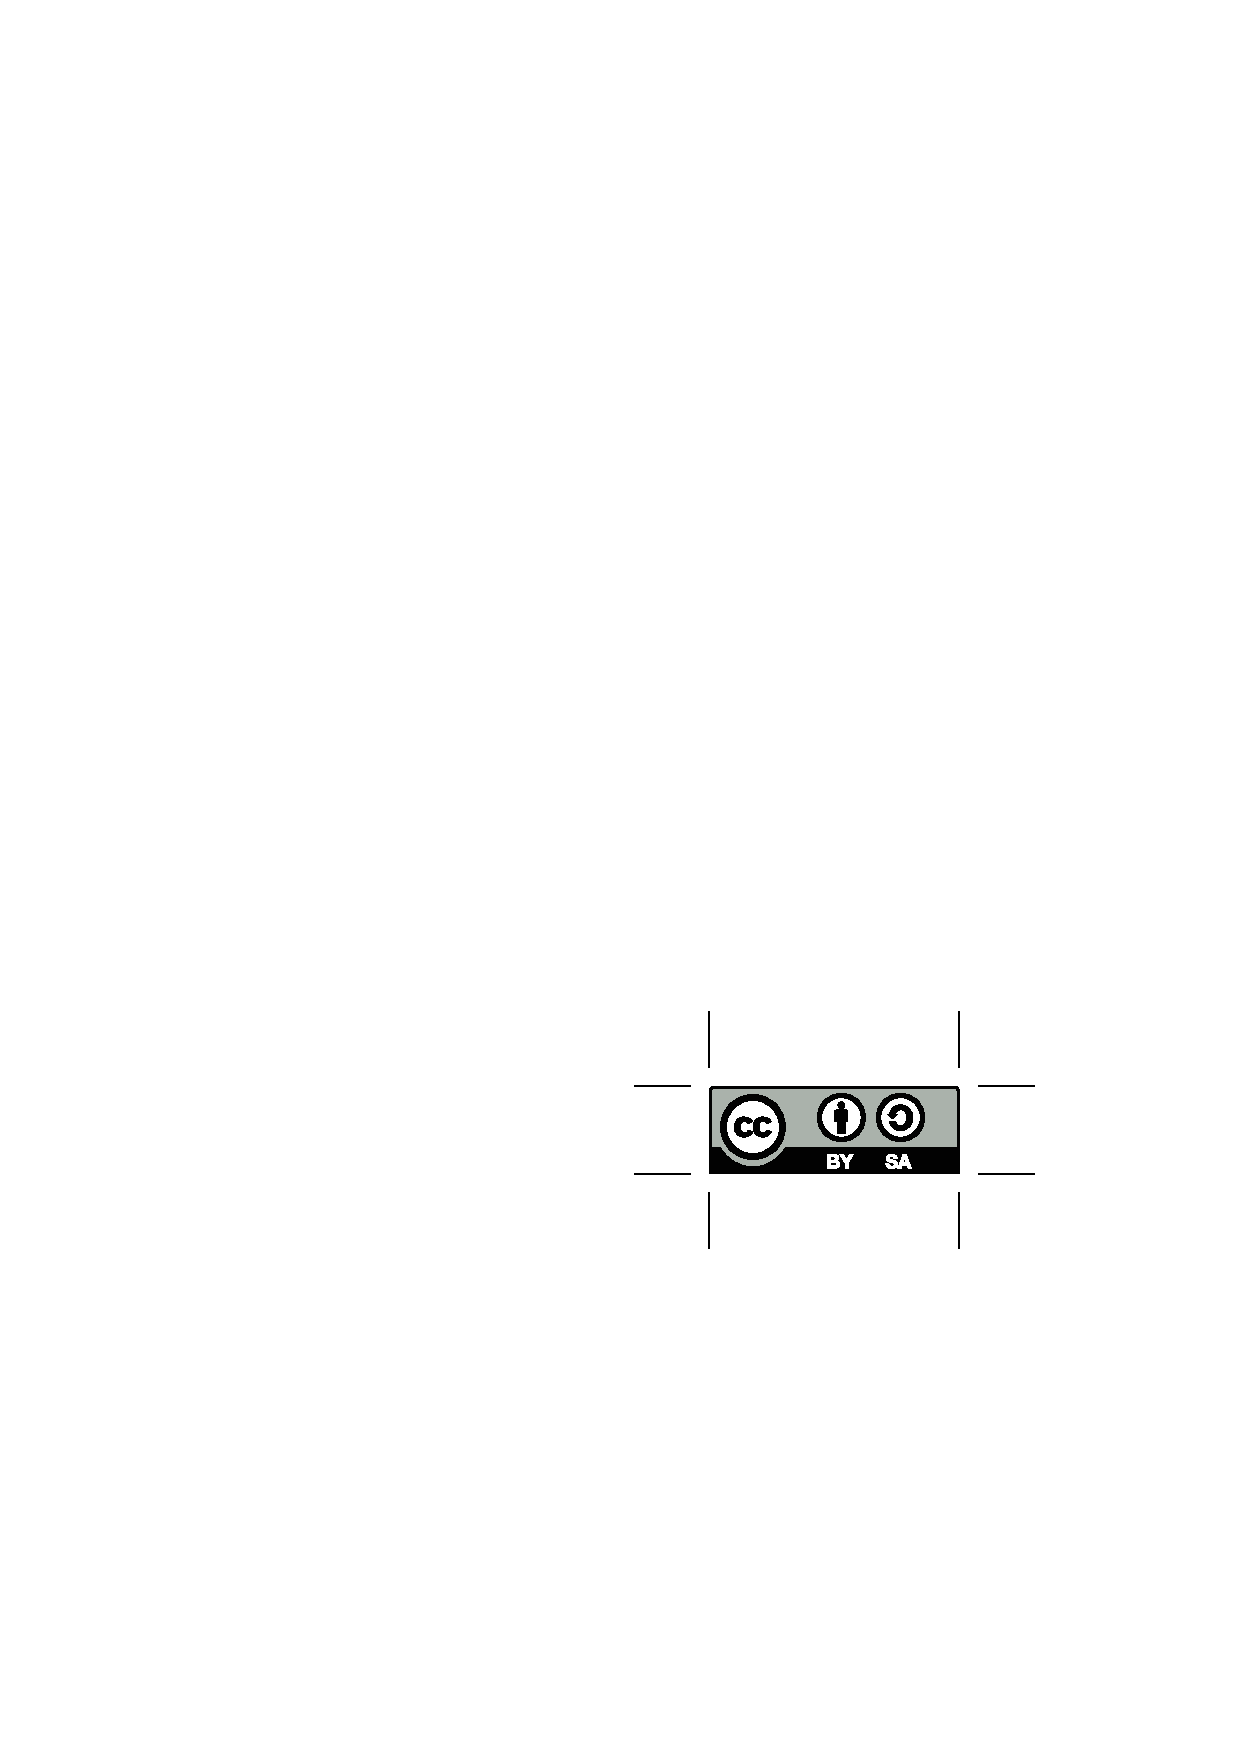
\includegraphics[scale=1]{by-sa} %
    \end{center} %
    
    Este trabajo titulado \emph{\thesisFlatTitle{}} por \thesisAuthor{}, se
    encuentra bajo la Licencia Creative Commons
    \href{http://creativecommons.org/licenses/by-sa/4.0/?ref=chooser-v1}%
    {Atribución-ShareAlike 4.0 International}.
    
    Para ver una copia de esta Licencia, visite
    \url{http://creativecommons.org/licenses/by-sa/4.0/}.\bigskip
    
    \copyright \the\year \hfill%
    \thesisAuthor \hfill%
    \thesisInstitution
  }
}

  
  % Hoja de depuración, con comandos definidos por la plantilla.
  % \phantomsection
\pdfbookmark[1]{Debug}{Debug}

Esta es una página de depuración, para ver todos los comandos
definidos en config.tex

De \verb+babel+ se obtiene que \verb+\tablename+ es \tablename.  Por
lo tanto, en esta versión se usará ``\latabla'' para denotar a cada
``\tabla''.  Ver \tabref{tab:comandostab} para la lista de comandos
existentes.



Este documento es elaborado por \thesisAuthorAddress~\thesisAuthor\
(\thesisAuthorShort) con carné \thesisAuthorTECID, para optar por el
título de \thesisAuthorDegree.

\genderAsesor\ \nameAsesor.

\genderLectorI\ \nameLectorI.

\genderLectorII\ \nameLectorII.

Titulo crudo:

\begin{center}
  \thesisTitle.  
\end{center}

Título aplanado:

``\thesisFlatTitle''.

Palabras clave: \thesisKeywords.

Fecha borrador: \thesisDraftDate

Fecha final: \thesisFinalDate





  
  \thispagestyle{empty}

\rule{10mm}{0pt}

\vfill

Declaro que el presente documento de tesis ha sido realizado enteramente
por mi persona, utilizando y aplicando literatura referente al tema e
introduciendo conocimientos y resultados experimentales propios.

En los casos en que he utilizado bibliografía he procedido a indicar las
fuentes mediante las respectivas citas bibliográficas.  En consecuencia,
asumo la responsabilidad total por el trabajo de tesis realizado y por
el contenido del presente documento.



\vspace*{8mm}

\begin{flushright}
  \thesisAuthor\par
  Cartago, \today\par
  Céd: 1-0123-0456
\end{flushright}

\cleardoublepage

%%% Local Variables: 
%%% mode: latex
%%% TeX-master: "main"
%%% End: 

  %% -------------------------------------------------
  %% Acta y hoja del tribunal
  %%
  %% Asegúrse de que las fechas de defensa de tesis sean las que aparecen
  %% en las actas.
  
  %% Para la Licenciatura en Ingeniería Electrónica:

  %%   Acá se colocan las dos actas como plantillas para ser firmadas
  %%   por el tribunal.

  %%   El acta de aprobación, dependiendo del tribunal, puede dejarla
  %%   en blanco en la tesis, para que el tribunal firme la tesis completa
  %%   sobre esta acta, o, si el tribunal lo decide, extrae la hoja
  %%   para que sea firmada "caligráficamente" por los miembros del tribunal.
  %%   Al acta firmada, en formato PDF (ya sea firmado con tabletas gráficas o
  %%   en papel y escaneada) la integra al documento con el comando para incluir
  %%   el pdf directamente \includepdf{archivo} 
  %% ESTE ARCHIVO DEBE ELIMINARSE DE LA VERSIÓN FINAL

\thispagestyle{empty}

\begin{center}
  \begin{tabular}{c}
    \thesisInstitution \\
    \thesisDepartment \\
    Trabajo Final de Graduación \\
    Acta de Aprobación
  \end{tabular}
\end{center}

\vfill

\begin{center}
  \begin{tabular}{c}
    Defensa de Trabajo Final de Graduación \\
    Requisito para optar por el título de \thesisAuthorDegree\ en Electrónica\\
    Grado Académico de Licenciatura
  \end{tabular}
\end{center}

\vfill

%% \thesisAuthorAddress, \thesisAuthor y \thesisTitle están en main.tex
El Tribunal Evaluador aprueba la defensa del trabajo final de graduación
denominado \textsl{\thesisFlatTitle{}}, realizado por
%
\thesisAuthorAddress\ \thesisAuthor\ %
%
y, hace constar que cumple con las normas
establecidas por la \thesisDepartment{} del \thesisInstitution{}.

\vfill

\begin{center}
 Miembros del Tribunal Evaluador
\end{center}

\vfill

\begin{center}
  \begin{tabularx}{\textwidth}{cXc}
    \rule{0.45\textwidth}{0.5pt} && \rule{0.45\textwidth}{0.5pt} \\
    \nameLectorI                 && \nameLectorII \\
    \genderLectorI               && \genderLectorII
  \end{tabularx}
  
  \vspace{10mm}

  \begin{tabular}{c}
    \rule{0.45\textwidth}{0.5pt} \\
    \nameAsesor \\
    \genderAsesor
  \end{tabular}
\end{center}

\vfill

\begin{center}
  Cartago, \ifdraft{\thesisDraftDate}{\thesisFinalDate}\par
\end{center}

\cleardoublepage

%%% Local Variables: 
%%% mode: latex
%%% TeX-master: "main"
%%% End: 
  % Remover en versión final
  %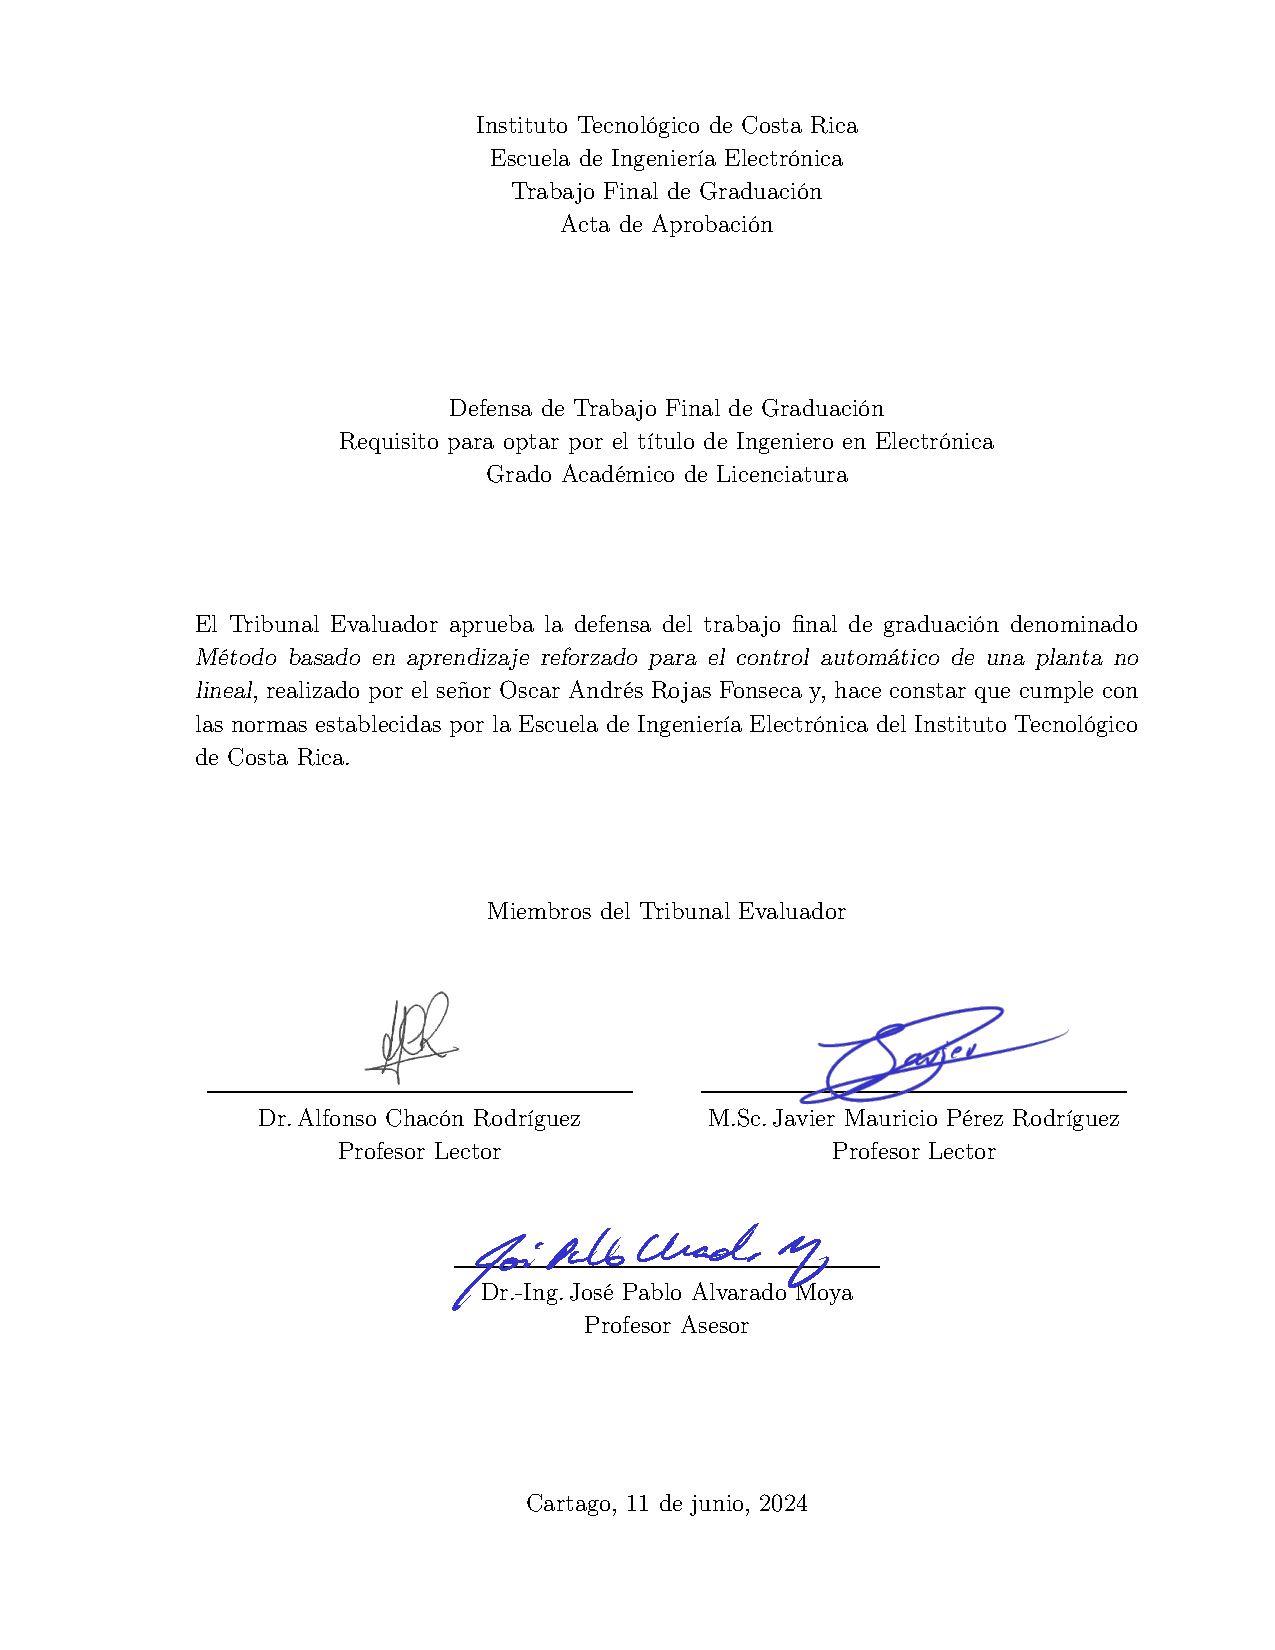
\includepdf{acta_aprob_firmada} % Incluir el acta firmada acá.

  %% El acta de evaluación usualmente la extrae del documento y
  %% la entrega al tribunal para que sea firmada, y ellos la hacen
  %% llegar al profesor del curso de TFG.  Ese documento no
  %% debe aparecer en la tesis final, así que esta línea deberá
  %% comentarla en la versión final:
  %% ESTE ARCHIVO DEBE ELIMINARSE DE LA VERSIÓN FINAL


\thispagestyle{empty}

\begin{center}
  \begin{tabular}{c}
    \thesisInstitution \\
    \thesisDepartment \\
    Trabajo Final de Graduación \\
    Tribunal Evaluador \\
    Acta de Evaluación
  \end{tabular}
\end{center}

\vfill

\begin{center}
  \begin{tabular}{c}
    Defensa del Trabajo Final de Graduación \\
    Requisito para optar por el título de \thesisAuthorDegree\ en Electrónica\\
    Grado Académico de Licenciatura
  \end{tabular}
\end{center}

\vfill

%% Configurar todo en config.tex
\begin{center}

  Estudiante:%
  \qquad \textbf{\thesisAuthor}%
  \qquad Carné: \thesisAuthorTECID

  \vspace*{2ex}

  \setlength\tabcolsep{0pt}
  \begin{tabular}{p{.25\textwidth}p{.73\textwidth}}
    Nombre del proyecto: & \textsl{\thesisFlatTitle}
  \end{tabular}
\end{center}
\vspace{5mm}

\vfill

Los miembros de este Tribunal hacen constar que este trabajo final de
graduación ha sido aprobado y cumple con las normas establecidas por
la \thesisDepartment{} del \thesisInstitution{} y es merecedor de la
siguiente calificación:

\vfill

\begin{center}
  Nota del Trabajo Final de Graduación: \rule{25mm}{0.5pt}
\end{center}

\vfill

\begin{center}
 Miembros del Tribunal Evaluador
\end{center}

\vfill

% Defina con \setLector* en main.tex (líneas 87-89) los lectores y asesor
\begin{center}
  \begin{tabularx}{\textwidth}{cXc}
    \rule{0.45\textwidth}{0.5pt} && \rule{0.45\textwidth}{0.5pt} \\
    \nameLectorI                 && \nameLectorII \\
    \genderLectorI               && \genderLectorII
  \end{tabularx}
  
  \vspace{10mm}

  \begin{tabular}{c}
    \rule{0.45\textwidth}{0.5pt} \\
    \nameAsesor \\
    \genderAsesor
  \end{tabular}
\end{center}

\vfill

\begin{center}
  Cartago, \ifdraft{\thesisDraftDate}{\thesisFinalDate}\par
\end{center}

\cleardoublepage

%%% Local Variables: 
%%% mode: latex
%%% TeX-master: "main"
%%% End: 
   % >> Remover en versión final <<
    
  %% Para la maestría en electrónica:
  %%% ESTE ARCHIVO DEBE ELIMINARSE DE LA VERSIÓN FINAL

\thispagestyle{empty}

\begin{center}
  \begin{tabular}{c}
    \thesisInstitution \\
    \thesisDepartment \\
    Proyecto de Graduación \\
    Tesis de Maestría \\
    Tribunal Evaluador
  \end{tabular}
\end{center}

\vfill

Tesis de maestría defendida ante el presente Tribunal Evaluador como
requisito para optar por el grado académico de maestría, del
\thesisInstitution.

\vfill

\vspace*{20mm}
\begin{center}
 Miembros del Tribunal
\end{center}
\vspace*{8mm}

\vfill

\begin{center}
  \begin{tabularx}{\textwidth}{cXc}
    \rule{0.45\textwidth}{0.5pt} && \rule{0.45\textwidth}{0.5pt} \\
    \nameLectorI                 && \nameLectorII \\
    \genderLectorI               && \genderLectorII
  \end{tabularx}
  
  \vspace{10mm}

  \begin{tabular}{c}
    \rule{0.45\textwidth}{0.5pt} \\
    \nameAsesor \\
    \genderAsesor
  \end{tabular}
\end{center}

\vfill


Los miembros de este Tribunal dan fe de que la presente tesis de
maestría ha sido aprobada y cumple con las normas establecidas por la
\thesisDepartment.

\vfill

\begin{center}
  Cartago, \today\par
\end{center}

\cleardoublepage

%%% Local Variables: 
%%% mode: latex
%%% TeX-master: "main"
%%% End: 
  % Remover en versión final
  %%% ESTE ARCHIVO DEBE ELIMINARSE DE LA VERSIÓN FINAL


\thispagestyle{empty}

\begin{center}
  \begin{tabular}{c}
    \thesisInstitution \\
    \thesisDepartment \\
    Tesis de Maestría \\
    Acta de Evaluación
  \end{tabular}
\end{center}

\vfill

Tesis de maestría defendida ante el presente Tribunal Evaluador como
requisito para optar por el grado académico de maestría, del
\thesisInstitution.

\vspace*{15mm}

%% Configurar todo en config.tex
\begin{center}
  Estudiante: \thesisAuthor
\end{center}

\vfill

\begin{center}
  Nombre del Proyecto: \thesisFlatTitle}
\end{center}

\vspace*{20mm}
\begin{center}
 Miembros del Tribunal Evaluador
\end{center}
\vspace*{8mm}

\vfill

% Los nombres de lectores y asesor se definen en el archivo main.tex
\begin{center}
  \begin{tabularx}{\textwidth}{cXc}
    \rule{0.45\textwidth}{0.5pt} && \rule{0.45\textwidth}{0.5pt} \\
    \nameLectorI                 && \nameLectorII \\
    \genderLectorI               && \genderLectorII
  \end{tabularx}
  
  \vspace{10mm}

  \begin{tabular}{c}
    \rule{0.45\textwidth}{0.5pt} \\
    \nameAsesor \\
    \genderAsesor
  \end{tabular}
\end{center}

\vfill

Los miembros de este Tribunal dan fe de que la presente tesis de
maestría ha sido aprobada y cumple con las normas establecidas por la
\thesisDepartment.

\vfill

\begin{center}
  Nota final de la Tesis de Maestría: \rule{3cm}{0.5pt}
\end{center}
\vfill

\begin{center}
  Cartago, \today\par
\end{center}

\cleardoublepage

%%% Local Variables: 
%%% mode: latex
%%% TeX-master: "main"
%%% End: 
   % Remover en versión final
  %% -------------------------------------------------
  \chapter*{Resumen}
\thispagestyle{empty}


La aplicación del aprendizaje reforzado en áreas de control automático representa un paso en la dirección de optimización de tareas que requieren capacidades de autonomía y flexibilidad, rubros que el RL ofrece con métodos como el DQN y el PPO, en su implementación con redes neuronales artificiales. El presente proyecto explora estos métodos en una planta de péndulo amortiguado de motor con hélice, con una estrategia que recompensa el bajo error angular y baja velocidad terminal. Se emplearon entornos virtuales para las pruebas de entrenamiento de control. Se evidencia la necesidad de ajustes en la función de recompensa para dar con el punto de control deseado y acercarse a cumplir con criterios usuales de control.


\bigskip

%% Defina las palabras clave con defKeywords en config.tex:
\textbf{Palabras clave:} \thesisKeywords

\clearpage
\chapter*{Abstract}
\thispagestyle{empty}

The application of reinforced learning in areas of automatic control represents a step in the direction of optimization of tasks that require autonomy and flexibility capabilities, items that RL offers with methods such as DQN and PPO, in its implementation with artificial neural networks. The present project explores these methods in a damped pendulum propeller motor plant, with a strategy that rewards low angular error and low terminal velocity. Virtual environments were used for control training tests. The need for adjustments to the reward function to find the desired control point and come close to meeting the usual control criteria is evident.

\bigskip

\textbf{Keywords:} Reinforcement learning, DQN, PPO, reward function, automatic control

\cleardoublepage

%%% Local Variables: 
%%% mode: latex
%%% TeX-master: "main"
%%% End: 

  \vspace*{0.4\textheight}
% No debe confundirse la dedicatoria con el agradecimiento.
% La dedicatoria solo tiene una línea corta de la persona a quien se dedica.

{\hfill{\Large{\emph{a mis queridos abuelos}}}}

  \chapter*{Agradecimientos}
\thispagestyle{empty}

El resultado de este trabajo no hubiese sido posible sin el apoyo de mis padres, Oscar Rojas Arce y Miriam Fonseca Elizondo, que día a día trabajaron para darme el estudio y los valores que tanto los caracterizan y me formaron como persona responsable y agradecida.

Agradecer a mi pareja Heikel Oporto Montero, por su paciencia y apoyo constante durante todo mi estudio universitario, que sin su presencia todo sería muy dificil de sobrellevar.

Agradezco a mis abuelos, Jose Miguel Fonseca Fonseca y Cristina Elizondo Pérez, que ya no se encuentran conmigo pero los recordaré con mucho cariño por su presencia durante toda mi infancia y valores sobresalientes.

Agradecer a los profesores de la Escuela de Ingeniería en Electrónica por su trabajo duro y apoyo en todos los trabajos realizados, especialmente al profesor José Pablo Alvarado Moya por su paciencia, sabiduría y calidad de docente.

\vspace*{1cm}

\thesisAuthor

Cartago, \today

\cleardoublepage

%%% Local Variables: 
%%% mode: latex
%%% TeX-master: "paMain"
%%% End: 


  %----------------------------------------------------------------------------
  \frontmatter
  %----------------------------------------------------------------------------
  \pagestyle{fancy}
  \pagenumbering{roman}

  \pdfbookmark[1]{Indice General}{Indice General}

  \parskip0ex                           % space between paragraphs

  \tableofcontents                      % Table of contents
  \listoffigures                        % List of figures
  \listoftables                         % List of tables

\ifdraft{%
  % todo's                              % TODOs
  \listoftodo
}{%
}

  %% ---------------------------------------------------------------------------
%% paNotation.tex
%%
%% Notation
%%
%% $Id: paNotation.tex,v 1.15 2004/03/30 05:55:59 alvarado Exp $
%% ---------------------------------------------------------------------------

\cleardoublepage
\renewcommand{\nomname}{Lista de símbolos y abreviaciones}
\setlength{\nomitemsep}{-\parsep}

%%
% Commands required for the nomenclature groups
%
% There are following prefix forms:
%  a   abbreviation    \syma[key]{symbol}{description}
%  g   general         \symg[key]{symbol}{description}
%%

\renewcommand{\nomgroup}[1]{%
  \ifthenelse{\equal{#1}{G}}{\section*{\hspace*{-\leftmargin}Notación general}}{}%
  \ifthenelse{\equal{#1}{A}}{\section*{\hspace*{-\leftmargin}Abreviaturas y Siglas}}{}%
}

\newcommand{\syma}[3][foo]{%
  \ifthenelse{\equal{#1}{foo}}%
  {\nomenclature[A]{#2}{#3}}{\nomenclature[A#1]{#2}{#3}}}
\newcommand{\symg}[3][foo]{%
  \ifthenelse{\equal{#1}{foo}}%
  {\nomenclature[G]{#2}{#3}}{\nomenclature[G#1]{#2}{#3}}}

%%
% Símbolos en la notación general
% (es posible poner la declaración en el texto
%%


%\symg[t]{$\sys{\cdot}$}{Transformación realizada por un sistema.}
\symg[yscalar]{$y$}{Escalar.}
%\symg[zconjugado]{$\conj{z}$}{Complejo conjugado de $z$.}
%\symg[rcomplexreal]{$\Re(z)$ o $z_{\Re}$}{Parte real del número complejo $z$.}
%\symg[icompleximag]{$\Im(z)$ o $z_{\Im}$}{Parte imaginaria del número
%                                        complejo $z$.}
%\symg[jimaginario]{$j$}{$j=\sqrt{-1}$.}
\symg[xvector]{$\mathbf{x}$}{Vector. \newline\hspace{1mm}%
  $\mathbf{x}=\left[ x_1 \; x_2 \; \ldots \; x_n \right]^T =
  \begin{bmatrix}
    x_1 \\ x_2 \\ \vdots \\ x_n
  \end{bmatrix}$}

\symg[mmatrix]{$\mat{A}$}{Matriz. \newline\hspace{1mm}%
  $\mat{A} =
  \begin{bmatrix}
    a_{11} & a_{12} & \cdots & a_{1m}\\
    a_{21} & a_{22} & \cdots & a_{2m}\\
    \vdots & \vdots & \ddots & \vdots\\
    a_{n1} & a_{n2} & \cdots & a_{nm}\\
  \end{bmatrix}$}

%\symg[C]{$\setC$}{Conjunto de los números complejos.}

%%
% Algunas abreviaciones
%%

\syma{IA}{Inteligencia Artificial}
\syma{RL}{Aprendizaje Reforzado}
\syma{SIP-Lab}{Laboratorio de Procesamiento de Imágenes y Señales}
\syma{DQN}{\textit{Deep Q-Network}}
\syma{DQL}{\textit{Deep Q-Learning}}
\syma{PPO}{Optimización de Política Próxima}
\syma{ITCR}{Instituto Tecnológico de Costa Rica}
\syma{PAMH}{Péndulo Amortiguado de Motor con Hélice}
\syma{RNAM}{Red Neuronal Artificial Mimetizadora}
\syma{RNA}{Red Neuronal Artificial}
\syma{PWM}{Modulación por Ancho de Pulso}
\syma{ReLU}{Unidad Lineal Rectificada}
\syma{MDP}{Procesos de Decisión de Markov}






\printnomenclature[20mm]

%%% Local Variables:
%%% mode: latex
%%% TeX-master: "paMain"
%%% End:
                    % Abbreviation

  \parskip1.3ex                         % space between paragraphs

  %----------------------------------------------------------------------------
  \mainmatter
  %----------------------------------------------------------------------------
  % where to look for graphics
  \graphicspath{{./}{./fig/}}
  %\pagenumbering{arab}

  % Main files
  %% ---------------------------------------------------------------------------
%% intro.tex
%%
%% Introduction
%%
%% $Id: intro.tex 1477 2010-07-28 21:34:43Z palvarado $
%% ---------------------------------------------------------------------------

$********************************************$\\
\textbf{Alfonso Chacón} 

\textit{Definición de problema a resolver y enfoque de solución}
Problema un poco abierto quizás pero claro. 
A como está planteado, puede disputarse si la elección de un método de aprendizaje reforzado es la óptima (algo igual no tan relevante). ¿Qué se gana con usar un método como los propuestos en un problema ya resuelto por métodos clásicos? 
¿Más allá de la obvia consderación didáctica? (o simplemente: lo hacemos porque lo podemos hacer). Considero conveniente contestar esta pregunta de manera explícita en el desarrollo del proyecto.

\textit{Objetivos y otros}
Objetivo general: Adecuado. Se puede mejorar dándole un poco más de especificidad, es decir, aclarar que el método a usar es DRL. Pero nada serio.

\textit{Redacción}
Buena. Algunos detalles de titulación mínimos (en español, solo se capitulan la primera letra del título y los nombres propios en los mismos).

\textit{Criterio: Aprobado  27/02/2024}

$********************************************$\\
\textbf{Javier Pérez}

\textit{Entorno del problema}
El Entorno del problema es muy largo, hay mucho texto que no es necesario para entender las circuinstancias del proyecto. Sea más directo.

\textit{Planteamiento del problema}
Los dos primeros párrafos del Planteamiento del problema es más parte de un marco teórico.

\textit{Soluciones}
La redacción de las posibles soluciones y Selección de la solución se vuelve confusa por momentos.
El diagrama que pone de la solución es más bien un esquema de la secuencia de pasos que se realizarán. No es lo mismo.

\textit{Criterio: Aprobado  05/02/2024}

$********************************************$\\

\chapter{Introducción}
\label{chp:intro}



\begin{comment}



\section{Entorno del proyecto}

El control automático de sistemas es una rama de la ingeniería que se dedica al diseño y análisis de sistemas de control que de manera automática buscan satisfacer criterios de optimalidad preestablecidos. Estos sistemas se utilizan en aplicaciones que abarcan desde el control de procesos industriales hasta el control de sistemas de navegación en vehículos autónomos, donde para lograr un control automático efectivo, se emplean técnicas y algoritmos, como el control proporcional-integral-derivativo (PID), el control adaptativo, el control moderno y otros \textcolor{SkyBlue}{ControlModerno}. La implementación de estos sistemas requiere del uso de hardware y software especializados, así como del conocimiento en áreas de la electrónica, informática y actualmente, la aplicación de la inteligencia artificial (IA) \textcolor{SkyBlue}{Kuo}.

El campo de aplicación de la IA está en constante crecimiento, impulsado por la necesidad de automatizar procesos y mejorar la eficiencia en diversas industrias. La IA se utiliza en sistemas de control para incrementar la precisión y velocidad de respuesta, apoyando así la toma de decisiones en tiempo real \textcolor{SkyBlue}{IntroSistemasControl} \textcolor{SkyBlue}{SistemaAlmidon}. Algunas de las aplicaciones más comunes incluyen la robótica, el control de procesos industriales, la domótica y la automatización de vehículos \textcolor{SkyBlue}{MarketResearch}. De acuerdo con un informe de Allied Market Research \textcolor{SkyBlue}{MarketResearch}, se espera que el mercado global de sistemas controlados mediante IA alcance los $\$ 30.8$ mil millones para el año 2026, con una tasa de crecimiento anual compuesta del $33.7\%$ desde 2019 hasta 2026. Se espera que la creciente demanda de soluciones de automatización, la evolución de esta tecnología y la creciente inversión en investigación y desarrollo impulsen aún más el crecimiento de este mercado en los próximos años \textcolor{SkyBlue}{MarketResearch}.

El fuerte aumento en la introducción del uso de IA en diversos ámbitos del mercado mundial, obliga a las universidades, a mantenerse activas en la propuesta y mejora de aplicaciones para la IA y su correspondiente divulgación. Esto se observa en la tendencia de investigaciones de las universidades líderes en tecnología a nivel mundial, como el Massachusetts Institute of Technology (MIT), la Universidad de Stanford, la Universidad de Oxford, entre otras \textcolor{SkyBlue}{UniversidadesIA}. Los experimentos que se realizan incluyen el desarrollo de algoritmos de aprendizaje automático para analizar grandes conjuntos de datos y descubrir patrones y tendencias, la aplicación de técnicas para resolver problemas en campos tan diversos como la medicina, la ingeniería, las ciencias sociales, además de la investigación en el uso de estas herramientas para mejorar la eficacia de los sistemas educativos \textcolor{SkyBlue}{MachineLearning}. Estos proyectos no solo están ayudando a los estudiantes a adquirir habilidades valiosas y a estar mejor preparados para los desafíos del mundo laboral, sino que también están generando nuevas oportunidades de investigación y desarrollo en áreas clave. Algunos ejemplos son la utilización de redes neuronales para la predicción del rendimiento académico, detección de enfermedades, identificación de aves, reconocimiento de emociones, entre otros \textcolor{SkyBlue}{MachineLearning}.

Alineado con lo anterior, el SIPLab de la Escuela de Ingeniería Electrónica del Instituto Tecnológico de Costa Rica, busca desarrollar soluciones a problemas regionales y nacionales en el campo mencionado anteriormente, esto mediante proyectos de procesamiento de señales donde se integre el aprendizaje automático y sus aplicaciones, permitiendo que estudiantes y profesores incursionen en el tema de la inteligencia artificial y la apliquen en sus actividades academicas \textcolor{SkyBlue}{SIPLab}. 



\section{Planteamiento del problema}

\subsection{Generalidades}

En la actualidad, el incremento en la complejidad de las plantas de control y su variedad de componentes dificulta el diseño del controlador y su optimización. Una solución prometedora para este problema es la aplicación de técnicas de aprendizaje automático, específicamente el aprendizaje reforzado (RL), el cual permite que un sistema aprenda de su experiencia y adapte su comportamiento para lograr una tarea específica, esto gracias a un diseño eficiente en la toma de muestras de información, su interpretación y modelado respectivo. Este RL presenta una variedad considerable de métodos que posibilitan su clasificación en distintas categorías, siendo las principales el aprendizaje reforzado basado en un modelo y el aprendizaje reforzado sin modelo \textcolor{SkyBlue}{AprendRefor} \textcolor{SkyBlue}{DataScience}.

El RL como tal requiere tener un panorama claro del objetivo a cumplir para la correcta elección de métodos de aprendizaje congruentes y así, lograr optimizar el comportamiento de un agente en el entorno, donde los principales tipos de métodos de RL son: el RL basado en modelo (\textit{Model-based RL}, MBRL), RL sin modelo (\textit{Model-free RL}, MFRL) y el RL profundo (\textit{Deep RL}). El MBRL usa un modelo del entorno mediante el cual se aplican iteraciones de políticas o valores para el proceso, lo cual representa un enfoque más dirigido a la prueba y error en el entrenamiento del modelo con programación dinámica.  El MFRL efectua una relación más directa con el ambiente a controlar, únicamente basándose en experiencias obtenidas por contextualización como el caso de la aplicación de la función $Q$ con el \textit{Q-learning} o SARSA. El Deep RL combina los métodos anteriores con redes neuronales profundas, lo que le permite representar y procesar datos más complejos (alta dimensión) y mejorar el rendimiento del agente sin necesidad de extraer características manualmente del entorno \textcolor{SkyBlue}{DataScience}

En términos generales, para realizar un diseño de un controlador con aprendizaje reforzado es necesario el conocimiento en ingeniería en electrónica, en particular el diseño y construcción de sistemas electrónicos, teoría de sistemas, sistemas digitales, sensores y actuadores, de manera que se pueda garantizar la implementación eficiente, precisa y confiable que integre, además, técnicas del aprendizaje automático \textcolor{SkyBlue}{Control} \textcolor{SkyBlue}{BBVA} \textcolor{SkyBlue}{VideoIA}.

Como contexto para este proyecto, se parte del trabajo de Brenes Alfaro \textcolor{SkyBlue}{TesisJorge}, quien propuso un sistema basado en redes neuronales, para emular el comportamiento de una planta de laboratorio, específicamente el Péndulo Amortiguado a Hélice (PAMH), comúnmente utilizado en el Laboratorio de Control Automático de la Escuela de Ingeniería Electrónica del ITCR. Así, se cuenta con una red neuronal que se comporta de manera similar a la versión física de la planta, considerando perturbaciones y otros factores que definen el comportamiento de la planta real \textcolor{SkyBlue}{PAMHinfo}, y que permite entonces ser usada en enfoques libres de modelo para el diseño de controladores, usando técnicas de aprendizaje reforzado, sin arriesgar la integridad de la planta real, y permitiendo su uso en tiempo de simulación acelerado.

En este punto, se cuenta con un modelo del comportamiento de la planta de laboratorio PAMH. Sin embargo, no se ha propuesto aun ningún método de control basado en aprendizaje reforzado \textcolor{SkyBlue}{TesisJorge}, donde los métodos más comunes son basados en modelos y sin modelo. El primero presenta iteraciones con políticas o valores programados dinámicamente, mientras que el segundo se basa en cálculos de optimización con gradiente o libres de él. Además, se denomina el apartado de aprendizaje reforzado profundo (\textit{Deep RL}) como una combinación de los métodos mencionados \textcolor{SkyBlue}{DataScience}.

De esta manera, la problemática planteada desde el punto de vista ingenieril apunta a una premisa enfocada al aprendizaje automático aplicado mediante el RL para el control automático.

\subsection{Síntesis del problema}

Se carece de un sistema de control automático, que por medio de técnicas de aprendizaje reforzado, permita manipular el comportamiento de una planta de control no lineal.



\section{Enfoque de la solución}

Ahora que se conoce la problemática y el entorno de este proyecto que persigue aplicar el aprendizaje automático al control de una planta no lineal, es necesario plantear algunas opciones que permitan resolver dicho problema, las cuales se ven direccionadas a los métodos y algoritmos de aprendizaje existentes.

Así, se proponen tres alternativas que permiten el control de la planta PAMH (Figura \ref{fig:PAMH}) con diferentes frentes de operación de aprendizaje reforzado. Este tipo de aprendizaje en general mantiene una estructura como la mostrada en la Figura \ref{fig:EstructuraAR}.

\begin{figure}[h]
    \centering
    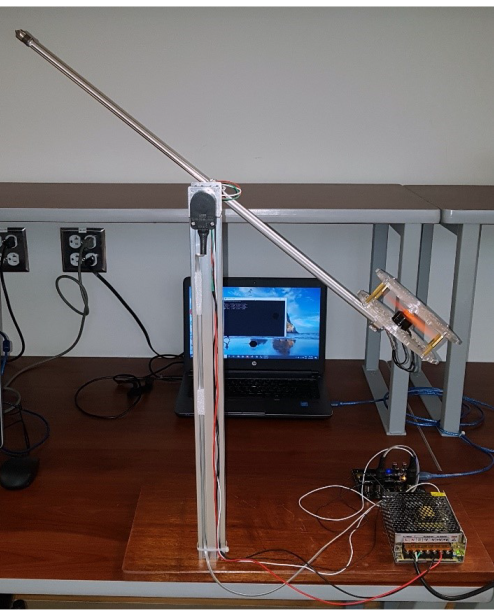
\includegraphics[width=0.3\textwidth]{fig/new/PAMH.png}
    \caption{Planta de laboratorio PAMH \textcolor{SkyBlue}{TesisJorge}.}
    \label{fig:PAMH}
\end{figure}

\begin{figure}[h]
    \centering
    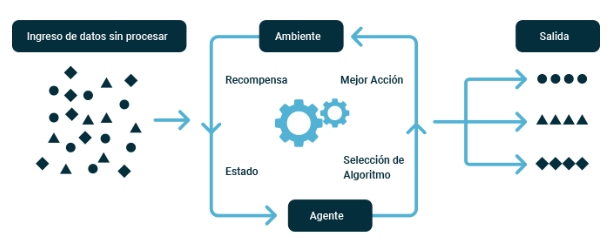
\includegraphics[width=0.6\textwidth]{fig/new/EstructuraAR.png}
    \caption{Modelo de aprendizaje reforzado \textcolor{SkyBlue}{FiguraEstructAR}.}
    \label{fig:EstructuraAR}
\end{figure}

Se realizó la respectiva valoración con una matriz de Pugh que expusiera los puntos a considerar para la elección de la alternativa.

\subsection{Solución 1}

Una red neuronal recurrente (\textit{Recurrent Neural Network}, RNN) presenta su mejor desempeño en el reconocimiento de la voz, donde las secuencias de datos son considerablemente grandes para obtener un entrenamiento eficiente de un modelo, ya que este recorre la trayectoria de los datos en el tiempo, donde cada punto representa un grado de optimización del modelo \textcolor{SkyBlue}{DataScience}.

\subsection{Solución 2} \label{SolucionSeleccionada}

Los métodos de aprendizaje reforzado profundo (\textit{Deep Reinforcement Learning}, DRL) presentan un aumento de la demanda y desarrollo en el área de control, de manera que permiten realizar cálculos complejos y representarlos de manera eficiente en espacios de estados de dimensiones altas, logrando un muy buen desempeño en tareas como el reconocimiento de imágenes \textcolor{SkyBlue}{DataScience}.

\subsection{Solución 3}

Métodos clásicos de aprendizaje reforzado como los cálculos basados en el gradiente o las iteraciones de políticas o valores pueden llegar a representar un camino claro para lograr comportamientos deseados en aplicaciones de control, donde se encuentran diferentes algoritmos que permiten optimizar el entrenamiento de los modelos al aplicar fórmulas específicas para cada método y comportamiento deseado \textcolor{SkyBlue}{DataScience}.


\subsection{Selección de la solución}

Como se observa, cada alternativa corresponde a un modelo de trabajo al aplicar el aprendizaje automático en el control de una planta de laboratorio PAMH, de manera que se considerarán aspectos en los que se evidencia la elección de la solución \ref{SolucionSeleccionada} como la más adecuada para el trabajo en cuestión, esto mediante las valoración en la matriz de Pugh del cuadro \ref{tab:MatrizPugh}.

\begin{table}[h]
\caption{Matriz de Pugh de las opciones de solución.}
\begin{tabular}{lcccc}
\hline
\multicolumn{1}{|c|}{\multirow{2}{*}{\textbf{Criterios}}} &
  \multicolumn{1}{c|}{\multirow{2}{*}{\textbf{Peso}}} &
  \multicolumn{3}{c|}{\textbf{Alternativas}} \\ \cline{3-5} 
\multicolumn{1}{|c|}{} &
  \multicolumn{1}{c|}{} &
  \multicolumn{1}{l|}{\textbf{Solución 1}} &
  \multicolumn{1}{l|}{\textbf{Solución 2}} &
  \multicolumn{1}{l|}{\textbf{Solución 3}} \\ \hline
\multicolumn{1}{|l|}{\begin{tabular}[c]{@{}l@{}}Fiabilidad de control del PAMH\end{tabular}} &
  \multicolumn{1}{c|}{4,5} &
  \multicolumn{1}{c|}{0} &
  \multicolumn{1}{c|}{+1} &
  \multicolumn{1}{c|}{+1} \\ \hline
\multicolumn{1}{|l|}{Costo económico} &
  \multicolumn{1}{c|}{4} &
  \multicolumn{1}{c|}{0} &
  \multicolumn{1}{c|}{+1} &
  \multicolumn{1}{c|}{-1} \\ \hline
\multicolumn{1}{|l|}{Tiempo de desarrollo} &
  \multicolumn{1}{c|}{3,5} &
  \multicolumn{1}{c|}{0} &
  \multicolumn{1}{c|}{+1} &
  \multicolumn{1}{c|}{-1} \\ \hline
\multicolumn{1}{|l|}{Código existente} &
  \multicolumn{1}{c|}{3} &
  \multicolumn{1}{c|}{+1} &
  \multicolumn{1}{c|}{+1} &
  \multicolumn{1}{c|}{+1} \\ \hline
\multicolumn{1}{|l|}{Optimización} &
  \multicolumn{1}{c|}{2,5} &
  \multicolumn{1}{c|}{-1} &
  \multicolumn{1}{c|}{+1} &
  \multicolumn{1}{c|}{0} \\ \hline
\multicolumn{1}{|l|}{Tiempo de entrenamiento} &
  \multicolumn{1}{c|}{2} &
  \multicolumn{1}{c|}{-1} &
  \multicolumn{1}{c|}{+1} &
  \multicolumn{1}{c|}{0} \\ \hline
\multicolumn{1}{|l|}{Datos de entrenamiento} &
  \multicolumn{1}{c|}{1,5} &
  \multicolumn{1}{c|}{0} &
  \multicolumn{1}{c|}{0} &
  \multicolumn{1}{c|}{+1} \\ \hline
\multicolumn{1}{|l|}{Innovación} &
  \multicolumn{1}{c|}{1} &
  \multicolumn{1}{c|}{+1} &
  \multicolumn{1}{c|}{+1} &
  \multicolumn{1}{c|}{+1} \\ \hline
 &
  \multicolumn{1}{l}{} &
  \multicolumn{1}{l}{} &
  \multicolumn{1}{l}{} &
  \multicolumn{1}{l}{} \\ \cline{1-1} \cline{3-5} 
\multicolumn{1}{|l|}{\textbf{Suma general}} &
  \multicolumn{1}{c|}{} &
  \multicolumn{1}{c|}{-0.5} &
  \multicolumn{1}{c|}{20.5} &
  \multicolumn{1}{c|}{2.5} \\ \cline{1-1} \cline{3-5} 
\multicolumn{1}{|l|}{\textbf{Ranking}} &
  \multicolumn{1}{c|}{} &
  \multicolumn{1}{c|}{3"o} &
  \multicolumn{1}{c|}{1"o} &
  \multicolumn{1}{c|}{2"o} \\ \cline{1-1} \cline{3-5} 
\end{tabular}
\label{tab:MatrizPugh}
\end{table}


Con base en la matriz de Pugh desarrollada en el cuadro \ref{tab:MatrizPugh}, se seleccionaron ocho variables que permitieron puntuar los criterios para cada posible solución. 

En primera, se cuenta con la fiabilidad del control del PAMH, eso debido a que algunos métodos no encajan muy bien con el enfoque del proyecto, por lo que es necesario reaccionar en primera instancia con los objetivos que suelen sumarse a cada solución, donde la solución 1 no suele relacionarse con el control de un sistema en específico \textcolor{SkyBlue}{DataScience}.

El costo económico va en función del tiempo de desarrollo, compuesto del entrenamiento y optimización del modelo en cuestión, por lo que el costo computacional y presencial a largos periodos de tiempo es significativo, todo esto frente al tiempo limitado disponible para la elaboración del trabajo final de graduación. 

Cada método presenta características complejas respecto a la implementación de los modelos de aprendizaje automático actuales, por lo que es de vital importancia disponer de referencias bibliográficas que permitan el acceso a códigos de prueba y así, realizar las modificaciones pertinentes, de manera que el constante desarrollo de métodos de aprendizaje automático cumple con este punto.

Dada la teoría y las características de cada solución presentada, la optimización de cada método equivale a diferentes grados de complejidad, donde la solución 1 requiere ajustes adicionales de la estructura para lograrlo, mientras que el caso de los métodos clásicos de RL y DRL permiten un ajuste más cercano a la experiencia y recompensa, en este caso resaltando la solución 2 por su enfoque directo al control de comportamientos \textcolor{SkyBlue}{DataScience}.

Respecto al tiempo de entrenamiento, la estructura secuencial de las RNN castiga especialmente este punto, además de la cantidad de datos de entrenamiento, mientras que el RL mejora este ámbito al aprovechar los recursos computacionales, especialmente el caso del DRL. Es así que los métodos clásicos de RL requieren menor cantidad de datos de entrenamiento pero mayor tiempo de iteración para optimizar, superado fácilmente por el DRL \textcolor{SkyBlue}{DataScience}.

Por último, al tratarse de un área de estudio en auge, constantemente se publican nuevos avances y métodos para cada tipo de modelo de aprendizaje automático, de manera que a nivel general cada solución significa innovación en sus estructuras.

Así y en suma, la solución con valor aceptable se trata de la número 2, donde el caso a utilizar se trata del aprendizaje reforzado profundo (DRL), por sus cualidades más enfocadas al problema en cuestión del proyecto.

En la Figura \ref{fig:Diagbloques} se muestra el diagrama de bloques de la solución propuesta, lo cual permite plantear un primer enfoque de la metodología a desarrollar.

\begin{figure}[!h]
    \centering
    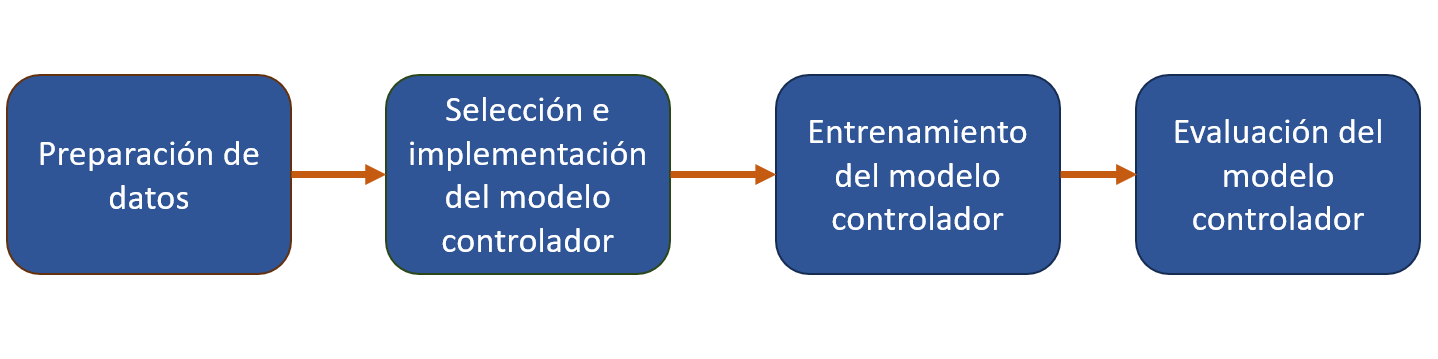
\includegraphics[width=0.7\textwidth]{fig/new/Diagbloques.png}
    \caption{Diagrama de bloques del proceso simplificado de aprendizaje reforzado profundo.}
    \label{fig:Diagbloques}
\end{figure}

\begin{comment}
Bajo dicha modalidad de trabajo se espera el cumplimiento de algunas condiciones necesarias para un correcto entrenamiento y validación del modelo a elaborar, las cuales se muestran en el cuadro \ref{tab:condiciones}
\end{comment}
Bajo dicha modalidad de trabajo se espera el cumplimiento de algunos requisitos necesarios para un correcto entrenamiento y validación del modelo a elaborar, los cuales se muestran en el cuadro \ref{tab:requisitos}

\begin{comment}
\begin{table}[!h]
\caption{Conjunto de condiciones mínimas necesarias para un entrenamiento eficiente del modelo.}
\label{tab:condiciones}
\centering
\begin{tabular}{|c|c|c|}
\hline
\centering\cellcolor{tableheader}\textcolor{white}{\textbf{Parámetro}} & \centering\cellcolor{tableheader}\textcolor{white}{\textbf{Entrenamiento}} & \cellcolor{tableheader}\textcolor{white}{\textbf{Validación y prueba}} \\ \hline
\textit{Conjunto de datos} & 500 episodios          & 100 episodios                \\ \hline
\textit{Duración}          & 3 segundos             & 3 segundos                   \\ \hline
\end{tabular}
\end{table}
\end{comment}


\begin{comment}
\begin{table}[!h]
\caption{Conjunto de requisitos para la comunicación del controlador mediante DRL.}
\label{tab:requisitos}
\centering
\begin{tabular}{|c|p{11cm}|}
\hline
\centering\cellcolor{tableheader}\textcolor{white}{\textbf{Número}} & {\centering\cellcolor{tableheader}\textcolor{white}{\textbf{Requisito}}} \\ \hline
$1$ & Sistema de captura lee el estado y aplica la acción en tiempo continuo. \\ \hline
$2$ & Sistema de captura de datos capaz de usarse con planta real y planta simulada. \\ \hline
$3$ & Sistema de captura puede acoplarse al controlador con señal de entrada y salida. \\ \hline
\end{tabular}
\end{table}



\section{Objetivo General}

Diseñar un sistema de aprendizaje automático para el control del ángulo de una planta no lineal PAMH.

\textbf{Indicador:} Sistema capaz de alcanzar un error angular inferior al $10\%$ frente a un estímulo constante. 

\subsection{Objetivos específicos}

\begin{enumerate}
    \item Seleccionar un método de aprendizaje reforzado apto para el control no lineal.

\textbf{Indicador:} Métrica de matriz de Pugh sobre métodos preseleccionados de aprendizaje reforzado.

    \item Diseñar la estrategia de captura de datos necesarios para el entrenamiento del modelo de aprendizaje reforzado que controle el modelo imitador del prototipo de laboratorio.

\textbf{Indicador:} Cumplimiento de los requisitos tabulados en el cuadro 2.

    \item Implementar el modelo de aprendizaje reforzado para el control del ángulo y entrenamiento del PAMH.

\textbf{Indicador:} Métrica de recompensa acumulada durante el proceso de entrenamiento y sistema entrenado que logra controlar el ángulo de la planta PAMH emulada.

    \item Evaluar el modelo de aprendizaje automático utilizado.

\textbf{Indicador:} Evaluación de al menos 5 configuraciones distintas de hiperparámetros del modelo seleccionado.


\end{enumerate}





\end{comment}

















\section{*************************************************}



%%% Local Variables: 
%%% mode: latex
%%% TeX-master: "main"
%%% End: 

  \chapter{Marco teórico}
\label{ch:teoria}

En el presente capítulo se repasan los conceptos que fundamentan el proceso de diseño de un controlador de una planta de laboratorio como el péndulo amortiguado a hélice, mediante prácticas de aprendizaje reforzado.

\section{Péndulo amortiguado de motor con hélice}

El péndulo amortiguado de motor con hélice (PAMH) se trata de un sistema extrapolado de un péndulo simple, compuesto de un motor con hélice, controlado por una señal de modulación por ancho de pulsos (\textit{pulse-width modulation}, PWM), una masa pequeña colocada en contrapeso al motor, el péndulo resultante de los brazos de aluminio y pesos correspondientes, así como soportes de aluminio de baja fricción, componentes responsables de mantener la estructura. Un modelo simplificado del sistema se muestra en la figura \ref{fig:modpen} junto con las magnitudes y vectores utilizados en la generación de modelo analítico del sistema \cite{PAMH1}.

\begin{figure}[h]
	\centering
	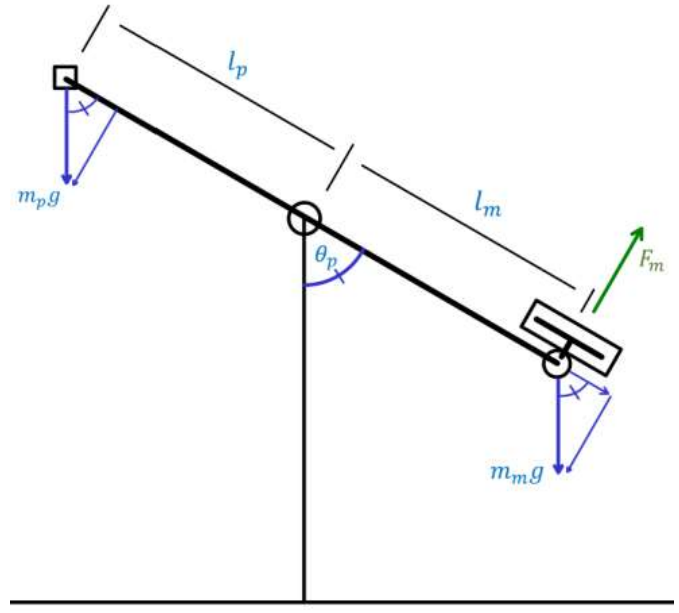
\includegraphics[scale=0.3]{fig/new/ModeloPendulo.png}
	\caption{Modelo simplificado del PAMH. Fuente: \cite{PAMHppt}}
	\label{fig:modpen}
\end{figure}

El objetivo principal  de dicho sistema es controlar la magnitud del ángulo $\theta_p$ medido entre la estructura y el péndulo, únicamente aplicando la señal PWM al motor que se encuentra a una distancia $l_m$ de la estructura y ejerce una fuerza $F_m$, que provoca el movimiento de su masa $m_m$ mientras, a una distancia de $l_p$ del centro, se encuentra una masa $m_p$ que contrarresta el movimiento.

\subsection{Modelo analítico del PAMH}

El modelado de sistemas físicos permite la elaboración de planes de trabajo con una base en común y bien sustentada en las características del entorno utilizado, permitiendo el diseño de controladores funcionales y eficientes. Este enfoque facilita la predicción del comportamiento del sistema bajo diversas condiciones operativas y la implementación de estrategias de control robustas, de manera que es común la elaboración de diagramas, como el caso de la figura \ref{fig:modpen} para la interpretación matemática \cite{Nise}.

El problema del péndulo suele ser abordado como un problema de leyes de Newton, donde se parte de la \textit{ley de movimiento rotacional de Newton} aplicada al modelo simplificado de la figura \ref{fig:modpen}.
\begin{equation}
\sum \tau = J_p\, \vec{a}
\label{ecu:sumatorques}
\end{equation}
La sumatoria de torques $\tau$ corresponde a la inercia del cuerpo péndulo $J_p$ por su aceleración ángular $\vec{a}$ \cite{Ogata}, de manera que la ecuación (\ref{ecu:sumatorques}) equivale a:
\[\tau_m - \tau_{mg} - \tau_{\beta} + \tau_{pg} = J_p \vec{a}\]
\begin{equation}
l_m\, F_m - l_m\, m_m g \,\sen(\theta_p)- l_m \,\beta \,\dot{\theta_p} + l_p\, m_p g\, \sen(\theta_p) = J_p\, \ddot{\theta_p}
\end{equation}
en donde $\beta$ corresponde a la constante de rozamiento en el eje central de la planta, constante comúnmente despreciable. Además, para deflexiones pequeñas se linealiza la ecuación con la aproximación $\sen(\theta_p) \approx \theta_p$. Las ecuaciones de estado son:
\[x_1 = \theta_p \qquad x_2 = \dot{\theta}_p \qquad y = x_1 = \theta_p\]
\begin{equation}
	\left \{ \begin{array}{lcc} \dot{x}_1 = x_2 \\ \\ \dot{x}_2 = -\dfrac{l_m \beta}{J_p} x_2 + (m_p l_p -m_m l_m)\dfrac{g}{J_p}x_1 +\dfrac{l_m}{J_p}F_m \end{array} \right.
	\label{ecu:sistemaPAMH}
\end{equation}
y la función de transferencia al aplicar el análisis en frecuencia:
\begin{equation}
T(s) = \frac{\theta_p(s)}{F_m(s)} = \frac{\dfrac{l_m}{J_p}}{s^2 + \dfrac{l_m\beta}{J_p}s +\dfrac{(l_m m_m-l_p m_p)g}{J_p}}
\end{equation}
punto desde el que se puede empezar a plantear alguna estrategia de control clásico al sistema o entorno, pero limitando al rango angular propiciado por la aproximación del componente trigonométrico.

Una consideración del procedimiento analítico realizado es que solo aproxima a la planta real, pues el modelo de la ecuación (\ref{ecu:sistemaPAMH}) no considera el movimiento mecánico producto de la holgura en el eje, o factores de resistencia mecánica por los cables eléctricos que toman la señal angular o llevan la energía al motor, o alteraciones con histéresis producto del movimiento de esos cables, factores que, acumulados, acarrean retos adicionales en el diseño de un controlador.

\section{Redes neuronales artificiales (RNA)}

Las RNA nacen de la experimentación para emular computacionalmente la capacidad del cerebro humano. El modelo usual de una neurona artificial se muestra en la figura \ref{fig:neurona} \cite{RNACaravaca}. Los valores de entrada $x_i$ se escalan por los pesos correspondientes $w_{ni}$, para luego sumarlos y transformarlos con la función de activación $\varphi(\cdot)$ (o también $f(\cdot)$), resultando en la salida \cite{RNACaravaca}:

\begin{equation}
y_i = \varphi \left(\sum^m_{j=1} w_{ij} x_j \right)
\label{ecu:neurona}
\end{equation}

\begin{figure}[h]
	\centering
	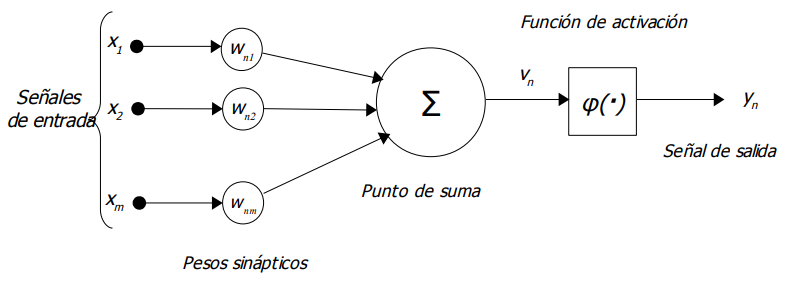
\includegraphics[scale=0.55]{fig/new/NeuronaRNA.png}
	\caption{Modelo de neurona artificial. Fuente: \cite{RNACaravaca}.}
	\label{fig:neurona}
\end{figure}

Un número $N$ de neuronas se interconecta dentro del sistema completo de la red neuronal artificial como se muestra en la figura \ref{fig:RNA}. Esta red recibe los vectores de entrada $\mathbf{x}$ y produce los vectores de salida $\mathbf{y}$. En el proceso, las capas ocultas producen los vectores $\mathbf{x}^{(n)}$ utilizando las matrices de pesos $\mathbf{A}_i$ que guardan los pesos correspondientes a cada neurona \cite{RNACaravaca} \cite{DataScience}.

\begin{figure}[h]
	\centering
	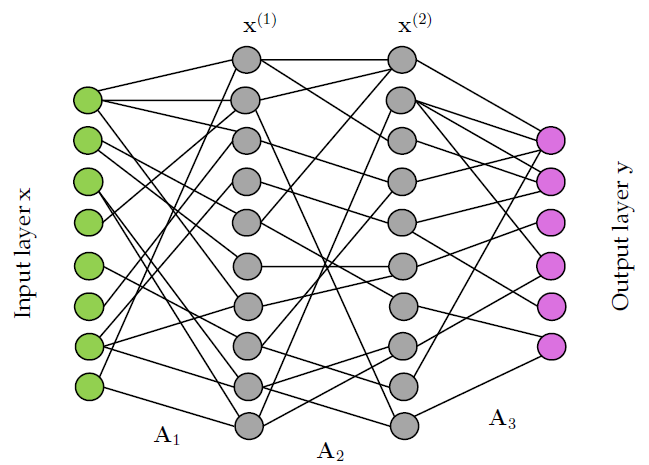
\includegraphics[scale=0.5]{fig/new/RNA.png}
	\caption{Modelo red neuronal artificial. Fuente: \cite{DataScience}.}
	\label{fig:RNA}
\end{figure}

Por lo tanto, la salida de una capa es entonces:

\begin{equation}
\mathbf{x}^{(n+1)} = f(\mathbf{A}, \mathbf{x}^{(n)})
\end{equation}

La red neuronal completa se modela con la composición de $M$ capas de la forma \cite{DataScience}:

\begin{equation}
\mathbf{y} = f_M \left( \mathbf{A}_M ,... , f_2 (\mathbf{A}_2, f_1(\mathbf{A}_1 , \mathbf{x}))  \right)
\end{equation}


La función de activación más utilizada en la actualidad, por el bajo costo computacional que representa, sumado a características teóricas que propician el funcionamiento correcto de los procesos de aprendizaje, es la llamada función ReLU \cite{DataScience}.

\begin{equation}
f_{ReLU}(x) = \left\{ \begin{array}{ll}
0 & \mbox{para $x \leq 0$} \\
x & \mbox{para $x > 0$}
\end{array}
\right.
\end{equation}

En síntesis, estos modelos neuronales tienen capacidad de aproximar cualquier función, ajustando el número de capas, el número de neuronas, y las funciones de activación. El objetivo con estos modelos es, dado un conjunto de entrenamiento con datos de entrada $\mathbf{x}$ para los que se conoce la salida $\mathbf{y}$, y dado un proceso de optimización, ajustar los pesos de cada capa, para que la diferencia entre las salidas que predice el modelo y las salidas $\mathbf{y}$ del conjunto de entrenamiento se minimice poco a poco, hasta que el sistema ``aprenda'' a reproducir esas predicciones, generalizando lo aprendido incluso a patrones de entrada no vistos durante el proceso de entrenamiento \cite{DataScience}.


\section{Aprendizaje reforzado}

En el aprendizaje reforzado (RL por sus siglas en inglés) se parte del supuesto que un agente debe aprender a interactuar en un entorno, de modo que a través de las acciones que el agente ejecuta en ese entorno, se maximice alguna función de recompensa. El agente tendrá algún estado que lo caracteriza (como su posición, su velocidad, etc.) y podrá realizar observaciones sobre el entorno, para decidir qué acciones tomar. Esto se ejemplifica en la figura \ref{fig:esquemaRL} \cite{DataScience}.

\begin{figure}[hh]
	\centering
	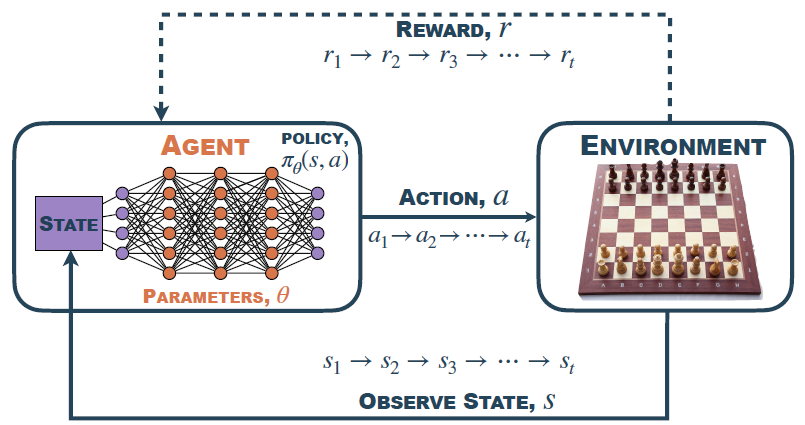
\includegraphics[scale=0.5]{fig/new/ReinforcementLearning.png}
	\caption{Etapas básicas del RL. Fuente: \cite{DataScience}.}
	\label{fig:esquemaRL}
\end{figure}

\subsection{Conceptos base del RL}

\subsubsection{Política}

En aprendizaje reforzado se conoce como política (\textit{policy}) a la estrategia que utiliza un agente para decidir qué acción $a$ tomar, dado su estado actual observable $s$. Existen varias formas de modelar las políticas. Por un lado, en los métodos de aprendizaje reforzado clásicos, la política es una función $\pi$ determinista que mapea de estados a acciones, mientras que métodos más recientes tienden a expresar la política como  \cite{DataScience}:
\begin{equation}
\pi (s,a) = Pr(a=a|\,\, s=s)
\label{ecu:policy}
\end{equation}
donde la política $\pi (s,a)$ es una función que expresa la probabilidad de tomar una acción $a$ dado un estado $s$.


\subsubsection{Recompensa}

La función de recompensa calcula a partir del estado actual del agente, y de la acción a tomar, una magnitud que indica qué tan bién está realizando el agente su tarea. Es la única realimentación que tiene el agente sobre su labor y es la única información disponible para que los algoritmos de aprendizaje reforzado decidan cómo deben mejorar esa recompensa.

Al maximizar las recompensas acumuladas, el agente puede determinar qué acciones son más beneficiosas para alcanzar objetivos a largo plazo. Por lo tanto, el diseño de una función de recompensa adecuada es esencial, ya que moldea el comportamiento del agente e impulsa el proceso de aprendizaje hacia los resultados deseados \cite{RLIntro}.

Una función de recompensa bien definida no solo anima al agente a alcanzar objetivos específicos, sino que también garantiza que el proceso de aprendizaje se mantenga estable y eficiente. Si la señal de recompensa es escasa o está mal definida, el agente tendrá dificultades para identificar patrones significativos a partir de sus interacciones, lo que conduce a comportamientos no deseados \cite{RLIntro}.


\subsubsection{Procesos de decisión de Markov (MDP)}

De manera simplicada, un $MDP$ es un formalismo para modelar un sistema en un estado específico de manera que la probabilidad de pasar a un nuevo estado depende únicamente del estado anterior del sistema y de la acción tomada \cite{DataScience}. 

De manera general, en un $MDP$ la dinámica del sistema se determina con las probabilidades de transición de un estado $s_k$ en el instante $k$ a un estado $s_{k+1}$ en el instante $k+1$ y con la acción $a_k$:
\begin{equation}
P(s', s, a) = Pr(s_{k+1}=s'\,|\, s_k=s, a_k=a)
\end{equation}

Los algoritmos clásicos de RL procuran aprender de la experiencia estas probabilidades y con ellas intentar maximizar la recompensa esperada en una sucesión óptima de estados y acciones. Este proceso es en general complejo, y por ello las técnicas modernas evitan tener que aprender la dinámica del sistema de forma explícita, y buscan formas en que solo implícitamente estas probabilides se aprendan \cite{DataScience}.

\subsubsection{Paso}

Un paso (\textit{step}) en el área de RL define la unidad básica de interacción entre un agente y su entorno. Tomando prestada la terminología de los sistemas de control, un paso se refiere a un único ciclo dentro del bucle de RL, como se muestra en la figura \ref{fig:esquemaRL}. Además, se describe en RL \cite{RLIntro}, el concepto, donde en cada paso, el agente realiza una acción en el entorno, observa el estado resultante y recibe una señal de recompensa, por lo que en un paso ocurre el intercambio de información entre los principales actores del proceso \cite{DataScience}.


\subsubsection{RL con redes neuronales}

Dado que las funciones de probabilidad que representan la dinámica del sistema, las políticas o incluso, en ocasiones, las mismas funciones de recompensa, deben aprenderse a partir de la experiencia del agente interactuando con su entorno, es natural que para estos procesos de aprendizaje se utilicen redes neuronales artificiales (RNA) como modelos de aproximación de esas funciones, aprovechando sus propiedades de aproximadores universales \cite{RLIntro}.

Las técnicas de aprendizaje reforzado que usan redes neuronales proponen entonces estrategias de recolección de los datos con los que se entrenará la red, los valores de referencia o funciones de pérdida que se utilizan para entrenar esas redes, y las estrategias de cómo usar los aprendizajes parciales mientras las redes aprenden en todo el proceso de interacción \cite{RLIntro}.

Como no se conoce lo que debe hacer un agente para mejorar sus espectativas de recompensa, se convierte en un reto plantear los problemas de entrenamiento de las redes neuronales, utilizando únicamente las recompensas o castigos a los comportamientos.


\subsubsection{Etapas de exploración y explotación}

Durante el entrenamiento de un agente por medio de aprendizaje reforzado, se debe asegurar mantener un balance entre las llamadas etapas de exploración y explotación \cite{RLIntro}.

La etapa de exploración incentiva al agente a tomar riesgos y elegir acciones aleatorias, solo para adquirir la experiencia de nuevas posibilidades de obtener mejores recompensas. En la etapa de explotación, el agente usa la política que ha aprendido previamente para determinar qué acciones tomar, con el riesgo de que sea muy conservador y no tome riesgos para aprender nuevas cosas, limitándolo a repetir experiencias que ya conoce \cite{RLIntro}. 

Los algoritmos o métodos de RL usualmente aplican la etapa de exploración al inicio de los entrenamientos de modelos para exponer al agente a situaciones que signifiquen una mayor recompensa. Con el avance del entrenamiento, se utilizan cada vez más las etapas de explotación, de modo que el agente aplica cada vez más las estrategias aprendidas para obtener su recompensa.

Una de las técnicas más utilizadas para lograr el balance entre la exploración y explotación en un entrenamiento se conoce como avaro-$\varepsilon$ (\textit{greedy-$\varepsilon$}). La técnica trabaja con una selección aleatoria, tal que con una probabilidad $\varepsilon$, el agente toma acciones aleatorias y con probabilidad $1-\varepsilon$ toma acciones dadas por la política aprendida \cite{RLIntro}.

El efecto del cambio de $\varepsilon$ se ejempifica en la figura \ref{fig:greedy_eps}, donde se aprecia la afectación de la selección de $\varepsilon$: un $\varepsilon=0$ (curva verde) provoca solo acciones aprendidas que no convergen a una recompensa máxima, mientras que el caso de $\varepsilon = 0.01$ y $\varepsilon = 0.1$ (curvas roja y negra, respectivamente) la exploración en ambas etapas resulta en una mejora progresiva de la recompensa. La velocidad de la convergencia hacia el máximo, varía asociado a qué tanto se le permite al agente explorar \cite{RLIntro}.


\begin{figure}[hh]
	\centering
	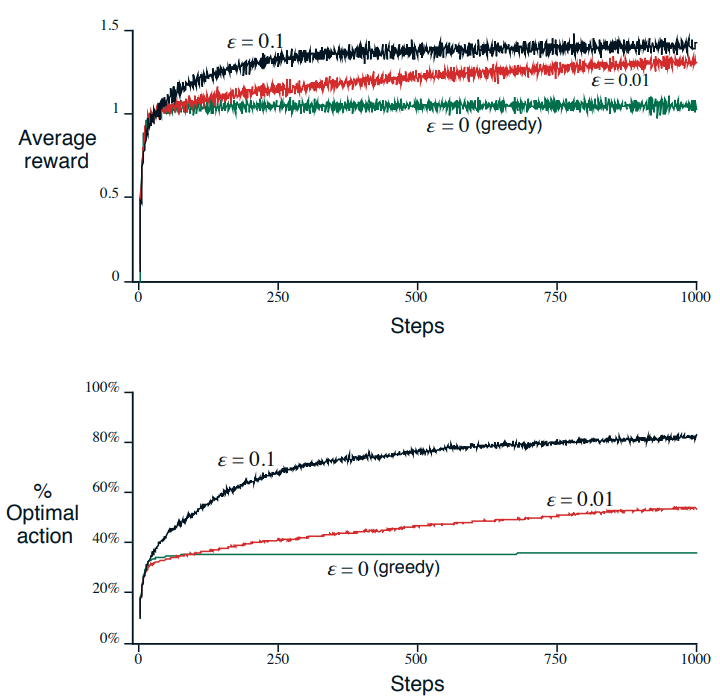
\includegraphics[scale=0.6]{fig/new/avaro_eps.png}
	\caption{Efecto de la selección de la probabilidad $\varepsilon$ en el desempeño del agente. Fuente \cite{RLIntro}.}
	\label{fig:greedy_eps}
\end{figure}


\subsubsection{Categorización del RL}

El RL dirige a los agentes a mejorar la recompensa en función de la política establecida para el control. Dada esa búsqueda del mejor desempeño en los entornos, se han propuesto numerosas técnicas o algoritmos para el RL, lo que se resume en la figura \ref{fig:RLcategorias}. Las categorías principales son: el RL basado en modelos y el libre de modelos. De igual forma se cuenta con el aprendizaje reforzado profundo (DRL), una combinación y reestructuración de métodos de cada subdivisión basada principalmente en las redes neuronales artificiales (RNA) con hasta cientos o miles de capas \cite{DataScience}.

\begin{figure}[hh]
	\centering
	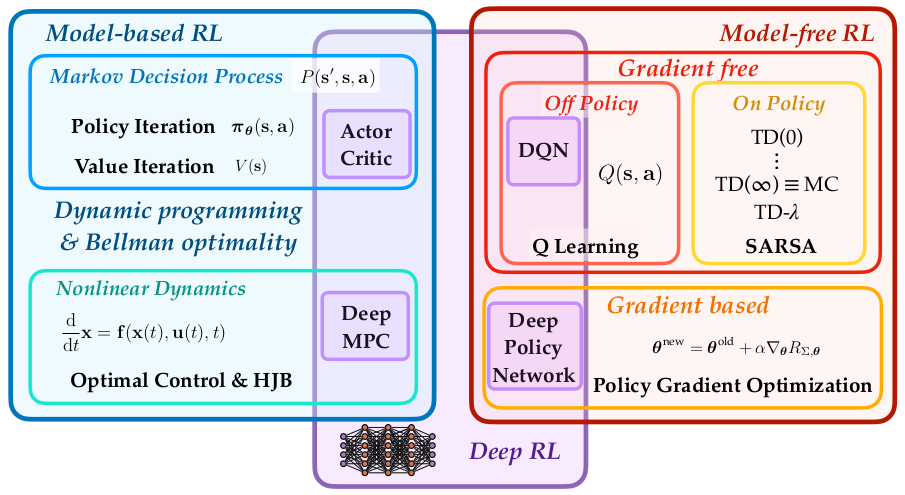
\includegraphics[scale=0.35]{fig/new/CatRL.png}
	\caption{Resumen de categorización del RL \cite{DataScience}.}
	\label{fig:RLcategorias}
\end{figure}

Cada método cuenta con sus premisas que los hacen adecuados para sistemas o entornos particulares, de manera que la identificación de los factores clave del entorno a controlar y su correcta caracterización permiten dirigir la selección de los métodos de RL. En esta ocasión se describen los algoritmos que se seleccionaron como posibles candidatos para el controlador del entorno PAMH.


\subsection{Deep Q-Network (DQN)}

El algoritmo (\textit{Deep Q-Learning}, DQL) es un método de aprendizaje reforzado introducido por la compañía DeepMind Technologies (hoy Google DeepMind) en el año $2013$. El DQL usa RNA para aproximar los llamados valores Q, por lo que se suele definir al método como DQN (\textit{Deep Q-Network}). El algoritmo de funcionamiento general del método se muestra en el apéndice \ref{apx:apendiceDQN} \cite{DQNbase}.

Los valores Q provienen del algoritmo clásico de aprendizaje Q (\textit{Q-learning}). Como se observa en la figura \ref{fig:RLcategorias}, se trata de un método fuera de política (\textit{off-policy}), de manera que el aprendizaje de un agente se realiza mediante la exploración de acciones que no siguen la política que haya aprendido el sistema \cite{DataScience}\cite{DQNexplained}. Se define el valor $V(s)$ en un estado $s$ como la recompensa esperada en el estado $s$, si se siguiera una política óptima a partir de allí, o en otras palabras, la mejor recompensa esperable a partir del estado $s$. El valor Q es similar, y se relaciona con el valor $V(s)$ con:
\begin{equation}
V(s) = \max_a Q(s,\,\, a)
\end{equation}

Es decir, el valor Q representa la recompensa total esperada al tomar una acción en un estado dado, siguiendo una política óptima a partir de allí.

\begin{comment}

En esos métodos clásicos se usa programación dinámica para su estimación, pero se requiere conocimiento de la llamada "dinámica del sistema", descrita a través de probabilidades de transición entre estados, dadas las acciones. pero dichas probabilidades suelen ser difíciles de determinar. Por eso aprendizaje Q opta por aproximar la estimación de Q con redes neuronales.

\end{comment}


Aprendizaje Q usa la técnica avaro-$\varepsilon$, de manera que con probabilidad $\varepsilon$ el algoritmo utiliza una acción $a_t$ aleatoria del espacio de acciones (exploración). Caso contrario, con probabilidad $1-\varepsilon$ se toma la acción directa de la respuesta de la RNA (explotación) con:
\begin{equation}
a_t = \arg \max_a Q^*(\phi(s_t), \,\, a;\,\, \theta)
\label{ecu:accionDQN}
\end{equation}
donde $\phi(s_t)$ es un mapeo del estado $s_t$ a un espacio de mayor dimensión y $\theta$ corresponde a los pesos de la estructura de la red neuronal. 

Las acciones y estados tomados se guardan en lotes para la valoración de sus recompensas respecto a la estimación de valores del lote, donde se les calcula una pérdida $L(\theta)$ para evaluar su desempeño con \cite{DQNbase}:
\begin{equation}
target_j = \left\{ \begin{array}{ll}
r_j & \mbox{para estado terminal $\phi_{j+1}$} \\
r_j + \gamma \,\, \max_{a'} Q(\phi_{j+1},\,\, a';\,\, \theta) & \mbox{para el resto $\phi_{j+1}$}
\end{array}
\right.
\end{equation}
\begin{equation}
L(\theta) = E \left[(target_j - Q(\phi_j,  \,\, a_j;\,\, \theta))^2\right]
\end{equation}
donde $target_j$ es la referencia objetivo del lote anterior y el término $Q(\phi_j,  \,\, a_j;\,\, \theta))$ corresponde a la predicción. Desde este punto es necesario aplicar el descenso de gradiente a la función de pérdida y actualizar los valores Q. Una cantidad $N$ de iteraciones aseguran la convergencia del modelo a los valores deseados y por ende, comportamientos deseados del entorno \cite{DataScience}\cite{DQNbase}.

\subsection{Optimización de política próxima (PPO)}

Se trata de un método basado en política (\textit{on-policy}) propuesto en $2017$ por la empresa OpenAI que aprende directamente a predecir la acción para espacios de estado discretos y continuos. Se busca cumplir una política definida y optimizarla poco a poco con actualizaciones. El método nace con la necesidad de utilizar un algoritmo de mayor accesibilidad en su implementación, al contrario de métodos similares pero de mayor complejidad, como el TRPO (\textit{trust region policy optimization}). El algoritmo del método PPO se muestra en el apéndice \ref{apx:apendicePPO} \cite{PPObase}. 

Entre las funciones clave del método PPO se encuentra la razón de los pesos de la política actual respecto a la anterior, con base en la función de política (\ref{ecu:policy}):
\begin{equation}
r_t (\theta) = \frac{\pi_\theta (a_t | \,\, s_t)}{\pi_\theta (a_{t_{old}} |\,\, s_t)}
\end{equation}
que evidencia el cambio respecto a la política anterior y su valoración por medio de la función de pérdida del aprendizaje:
\begin{equation}
L^{CLIP} (\theta) = \mathbf{E}_t \left[min (r_t (\theta) \,\, \mathbf{A}_t ,\,\, clip(r_t(\theta),\,\, 1-\varepsilon,\,\, 1+\varepsilon) \mathbf{A}_t)\right]
\label{ecu:lossPPO}
\end{equation}
donde $\varepsilon$ es un hiperparámetro del algoritmo que asegura que el cambio a la política anterior no sea muy abrupto para el proceso y el vector $\mathbf{A}_t$ corresponde al estimador de la función de ventaja, obtenido mediante la diferencia \cite{PPObase}:

\begin{equation}
\mathbf{A}_t = Q(s,a) - V(s)
\end{equation}

lo cual genera la recompensa ``extra'' que se puede obtener al tomar las acciones $V(s)$ sobre los valores $Q(s,a)$ \cite{PPOadv}.

En suma, a través de un número $N$ de iteraciones, el modelo pule poco a poco la política que va aprendiendo con cada cálculo de la pérdida (\ref{ecu:lossPPO}) y se actualizan los parámetros $\theta$ de la RNA que convergen durante el proceso para alcanzar la política óptima y maximizan la expectativa de recompensa \cite{DataScience}.

\section{Métricas de evaluación}

\subsection{Función de recompensa}

La función de recompensa sirve de guía a los agentes para decidir que acción tomar. Por consiguiente y de acuerdo con el comportamiento deseado, una función de recompensa engloba el objetivo, las preferencias y las restricciones que presenta la tarea, usualmente adquiriendo la información desde las observaciones al entorno e interpretándolas con base en el comportamiento deseado.

Por lo tanto a la hora de diseñar un sistema de RL, crear una función de recompensa y mantener el monitoreo en la misma, permite interpretar el comportamiento el agente y evaluar su desempeño, como en el ejemplo del caso en la figura \ref{fig:greedy_eps} con la recompensa de cada valor de $\varepsilon$ seleccionado \cite{DataScience}.

\subsection{Pérdida del modelo}

El valor de pérdida (\textit{loss}) en RL, como en el caso de la ecuación (\ref{ecu:lossPPO}), suele obtenerse de los cálculos de los gradientes o procesos de optimización, en donde una pérdida baja en RL no garantiza necesariamente un rendimiento óptimo. Principalmente indica que el agente está aprendiendo y mejorando su política basándose en la estructura de recompensas definida y en el algoritmo elegido \cite{DataScience}.

La principal métrica en RL suele ser la recompensa obtenida por el agente, dado que refleja directamente lo bien que el agente ha aprendido a maximizar sus recompensas, pero la pérdida también desempeña un papel crucial a la hora de guiar el proceso de aprendizaje para la actualización de políticas y funciones de valor.



\subsection{Error de posición angular}

Todo problema que incorpora secciones del control automático es evaluado mediante la respuesta a una entrada conocida a la que se le mide el error de estado estacionario, el tiempo de estabilización, el porcentaje de sobreimpulso, entre otros \cite{Nise}\cite{Ogata}.

Todo el proceso debe responder a una exigencia de punto de operación premeditado, en este caso un porcentaje de error de estado estacionario menor al $10\%$.
  \chapter{Control de PAMH basado en aprendizaje reforzado}
\label{ch:ControlPAMH}

Para obtener un modelo controlador de una planta como el péndulo amortiguado de motor con hélice, es necesario definir el modelo de RL a utilizar, el plan de entrenamiento del modelo y la función de recompensa que conduzca al comportamiento deseado del agente.

\section{Selección de modelos de RL}

En primera instancia se realiza una investigación biblográfica respecto a los métodos de RL comunmente utilizados para el control de entornos o sistemas similares a la planta PAMH, al igual que una búsqueda de repositorios o publicaciones realizadas para cada método de RL encontrado, de manera que cada uno de los métodos contara con un respaldo para la evaluación de los criterios seleccionados para la matriz de Pugh, mostrada la tabla \ref{tab:MatrizPugh}.

\begin{table}[h]
\centering
\caption{Matriz de Pugh de los métodos de RL candidatos.}
\begin{tabular}{lccccc}
\hline
\multicolumn{1}{|c|}{\multirow{2}{*}{\textbf{Criterios}}} &
  \multicolumn{1}{c|}{\multirow{2}{*}{\textbf{Peso}}} &
  \multicolumn{4}{c|}{\textbf{Alternativas}} \\ \cline{3-6} 
\multicolumn{1}{|c|}{} &
  \multicolumn{1}{c|}{} &
  \multicolumn{1}{l|}{\textbf{DQN}} &
  \multicolumn{1}{l|}{\textbf{PPO}} &
  \multicolumn{1}{l|}{\textbf{DDPG}} &
  \multicolumn{1}{l|}{\textbf{SAC}} \\ \hline
\multicolumn{1}{|l|}{\begin{tabular}[c]{@{}l@{}}Fiabilidad de control del PAMH\end{tabular}} &
  \multicolumn{1}{c|}{4} &
  \multicolumn{1}{c|}{0} &
  \multicolumn{1}{c|}{+1} &
  \multicolumn{1}{c|}{+1} &
  \multicolumn{1}{c|}{+1} \\ \hline
\multicolumn{1}{|l|}{Recursos computacionales} &
  \multicolumn{1}{c|}{3,5} &
  \multicolumn{1}{c|}{+1} &
  \multicolumn{1}{c|}{+1} &
  \multicolumn{1}{c|}{0} &
  \multicolumn{1}{c|}{-1} \\ \hline
\multicolumn{1}{|l|}{Tiempo de desarrollo} &
  \multicolumn{1}{c|}{3} &
  \multicolumn{1}{c|}{+1} &
  \multicolumn{1}{c|}{+1} &
  \multicolumn{1}{c|}{0} &
  \multicolumn{1}{c|}{0} \\ \hline
\multicolumn{1}{|l|}{Código existente} &
  \multicolumn{1}{c|}{2,5} &
  \multicolumn{1}{c|}{+1} &
  \multicolumn{1}{c|}{+1} &
  \multicolumn{1}{c|}{0} &
  \multicolumn{1}{c|}{0} \\ \hline
\multicolumn{1}{|l|}{Optimización} &
  \multicolumn{1}{c|}{2} &
  \multicolumn{1}{c|}{+1} &
  \multicolumn{1}{c|}{+1} &
  \multicolumn{1}{c|}{0} &
  \multicolumn{1}{c|}{0} \\ \hline
\multicolumn{1}{|l|}{Tiempo de entrenamiento} &
  \multicolumn{1}{c|}{1,5} &
  \multicolumn{1}{c|}{-1} &
  \multicolumn{1}{c|}{+1} &
  \multicolumn{1}{c|}{0} &
  \multicolumn{1}{c|}{+1} \\ \hline
\multicolumn{1}{|l|}{Innovación} &
  \multicolumn{1}{c|}{1} &
  \multicolumn{1}{c|}{-1} &
  \multicolumn{1}{c|}{0} &
  \multicolumn{1}{c|}{+1} &
  \multicolumn{1}{c|}{+1} \\ \hline
 &
  \multicolumn{1}{l}{} &
  \multicolumn{1}{l}{} &
  \multicolumn{1}{l}{} &
  \multicolumn{1}{l}{} \\ \cline{1-1} \cline{3-6} 
\multicolumn{1}{|l|}{\textbf{Suma general}} &
  \multicolumn{1}{c|}{} &
  \multicolumn{1}{c|}{8,5} &
  \multicolumn{1}{c|}{16,5} &
  \multicolumn{1}{c|}{5,0} &
  \multicolumn{1}{c|}{3.0} \\ \cline{1-1} \cline{3-6} 
\multicolumn{1}{|l|}{\textbf{Ranking}} &
  \multicolumn{1}{c|}{} &
  \multicolumn{1}{c|}{2"o} &
  \multicolumn{1}{c|}{1"o} &
  \multicolumn{1}{c|}{3"o} &
  \multicolumn{1}{c|}{4"o} \\ \cline{1-1} \cline{3-6} 
\end{tabular}
\label{tab:MatrizPugh}
\end{table}

La revisión de material respecto al algoritmo DQN se encuentra en el documento base del método \cite{DQNbase} publicado en el año $2013$ y los criterios o consideraciones importantes al respecto se encuentran en \cite{DQNexplained} y \cite{PytorchDQN}, como el problema de convergencia con espacios de acciones continuos \cite{ForoDQN}. En resumen, el método DQN cuenta con amplio respaldo de ejemplos de implementación en RL y presenta entrenamientos con resultados eficientes para espacios de acciones discretos y soluciones discretizadas.

En cuanto al método PPO, se consultó el documento base del método \cite{PPObase} publicado en el año $2017$ y de igual forma, repositorios y artículos sobre sus casos de aplicación, donde se demuestra su eficiencia al trabajar tanto con espacios de acciones discretos como continuos \cite{PPOyu} y \cite{PPOcoding2}.

El caso del método gradiente de política determinista profunda (DDPG, por sus siglas en inglés) publicado en el año $2019$, responde a una solución de los problemas del DQN con espacios continuos, en ocaciones conocido como DQN para espacios continuos. El algoritmo utiliza lógica del conocido DQL e implementaciones de políticas de igual forma \cite{DDPGbase}.

También se tiene el método actor-crítico blando (SAC, por sus siglas en inglés) publicado en el año $2018$, un algoritmo basado en RL de máxima entropía, pues el componente actor busca maximizar la recompensa esperada junto con la entropía, por lo que la convergencia a un comportamiento deseado es caracterizado por pasos ``suaves'' en lugar de saltos abruptos en acciones \cite{SACbase}.

El factor del recurso computacional requerido define el tiempo de entrenamiento o en algunos casos, la posibilidad de implementación del método. El DQN dispone de amplio repositorio de ejemplos, pero se trata del método de mayor antiguedad, por lo que no presenta el mismo enfoque de disminución de tiempos a costo de la capacidad de cálculo como si lo hicieron DDPG y SAC \cite{DDPGbase} \cite{SACbase}.

Por otro lado, los métodos DDPG y SAC al ser nuevos en comparación con los otros, no cuentan con el amplio registro de repositorios de implementación y pasos extra de optimización, mientras si cuentan con extensos algoritmos de funcionamiento, por lo que su tiempo de desarrollo se ve afectado.

El método PPO presenta las mejores cualidades para ser utilizado como algoritmo entrenador de un controlador para el entorno PAMH, descrito en el capítulo \ref{ch:teoria}. Como segunda posición se tiene el método DQN, por lo que se puede seleccionar de acuerdo con lo recomendado en las publicaciones referentes a su uso con discretización del espacio de acciones continuo.

\section{Preparación de entornos virtuales}

Dada la complejidad de los métodos de RL utilizados, el primer paso consiste en una implementación con entornos virtuales conocidos. La plataforma Gymnasium de Farama Fundation \cite{Gymnasium} ofrece una colección de entornos de código abierto disponibles para experimentación con estrategias de control. Los entornos consisten en simulaciones físicas de entornos particulares como péndulos simples y dobles, con actuadores y un conjunto de acciones predefinidas \cite{Gymnasium}.  

Luego del estudio de los algoritmos pertinentes para la aplicación del RL mediante PPO y DQN \cite{PPObase} \cite{DQNbase}, se aplican ajustes para funcionar, en primera fase, con entornos de acciones discretas, como es el caso del problema de control del péndulo invertido (\textit{CartPole}) \cite{Gymnasium}.

El segundo paso es adaptar el código para trabajar con entornos con características y mediciones de valores continuos. Como caso de estudio se usa el control del otro péndulo invertido (\textit{Pendulum}), en el cual se realizan las primeras pruebas de ajuste de ángulo objetivo, dado que el objetivo base del entorno es mantener el ángulo superior estático ($0^o$). Por lo tanto, el primer ajuste al método fue la implementación del error de ángulo:
\begin{equation}
E_{\theta} = |\theta - \theta_{objetivo}|
\label{ecu:errorangular}
\end{equation}
en lugar de únicamente el componente $\theta$ del péndulo en su función de recompensas, heredada del código base de Gymnasium \cite{Gymnasium}.

Para facilidad de acoplamiento de los modelos experimentales anteriores al caso concreto de PAMH, se adapta el modelo mimetizador del proyecto previo \cite{JorgeBrenes} a una interfaz de tipo Gymnasium, de manera que el modelo imitador del PAMH trabaje de forma similar a los modelos disponibles de RL que se usan en Gymnasium.

En las mediciones u observaciones al entorno simulado o real PAMH, hay un único valor observable: el ángulo del péndulo de la planta. Se adicionan parámetros de información para el procesamiento de la red neuronal para complementar el estado con aproximaciones de la primera derivada (como velocidad angular) de la forma:
\begin{equation}
\dot{\theta} = \theta_t - \theta_{t-1}
\end{equation}
y la segunda derivada (como aceleración):
\begin{equation}
\ddot{\theta} = \dot{\theta}_t - \dot{\theta}_{t-1}
\end{equation}
ambos casos basados en las diferencias entre los valores medidos en la actual iteracion $t$ y la anterior iteración $t-1$. 

Se agrega además a las observaciones el valor del ángulo objetivo $\theta_{objetivo}$, con la intención de que la red pueda aprender a inferir diferencias de comportamiento de la planta, dependientes del objetivo que esta deba alcanzar; pues no es lo mismo controlar para llegar a $10^o$ que a $90^o$. Por lo tanto, el vector utilizado de observación de la planta es:

\begin{equation}
obs_n = [\theta \, ,\quad \dot{\theta} \, ,\quad \ddot{\theta} \, ,\quad \theta_{objetivo}]
\label{ecu:observation}
\end{equation}

lo que corresponde al mapeo $\phi(s)$ de una dimensión a cuatro dimensiones, propuesto en este trabajo para cumplir la función introducida de forma general en la ecuación (\ref{ecu:accionDQN}).

\section{Parametrización de los modelos}

Uno de los puntos clave del trabajo realizado es el diseño de la función de recompensa enfocada en guiar al comportamiento deseado.

De igual forma, se presentan a continuación las configuraciones de los dos métodos seleccionados DQN y PPO.

\subsection{Función de recompensa}

La función de recompensa condiciona el comportamiento del agente por su relación directa con las características deseadas respecto a su comportamiento en el entorno.

Con base en los fundamentos relacionados a la planta PAMH, el problema definido para el agente es mantener un ángulo constante, indicado con anterioridad, además de alcanzar una velocidad angular baja, cuando se alcance el ángulo final.

Por lo tanto, se propone una ecuación que recompense alcanzar el ángulo deseado y caso contrario, castigar un ángulo diferente al deseado y una velocidad angular alta, pues este último indicaría que no se estabiliza el péndulo. La función propuesta se muestra en el algoritmo \ref{alg:reward}.

\begin{algorithm}[hh]
\caption{Función de recompensa}\label{alg:reward}
\begin{algorithmic}[1]
\State Recibe los componentes de la observación $\theta$, $\dot{\theta}$.
\State Recibe la señal de acción $PWM$ anterior $a_{t-1}$.
\State Recibe el ángulo objetivo $\theta_{objetivo}$.
\State Asegura el valor $\theta$ en radianes y en el rango $[-\pi,\pi]$.
\State Cálculo del error: 
\[E_{\theta} = |\theta - \theta_{objetivo}|\]
\State Potenciar y escalar el comportamiento no deseado con el costo por error angular $C_\theta$ y el costo por velocidad angular $C_{\dot{\theta}}$:
\[C_{\theta} = \theta^2_{error}\]
\[C_{\dot{\theta}} = 100 \cdot \dot{\theta}^2\]
\State Recompensa por comportamiento deseado:
\[R_{\theta} = 2 \cdot \left( e^{-C_{\theta}/\sigma_r} \, (1 - |C_{\dot{\theta}}|)\right)\]
\State Recompensa y castigo por señal de acción deseada:
\[E_{a_{t-1}} = \left\{ \begin{array}{ll}
0 & \mbox{para acción $0<|a_{t-1}|<0.25$} \\
20^{|a_{t-1} - 0.25|} & \mbox{para el resto de $a_{t-1}$}
\end{array}
\right.\]
\State La señal de recompensa resultante:
\[R = \min \left[-C_{\theta}, \,\, -E_{a_{t-1}}\right] + R_{\theta}\]
\end{algorithmic}
\end{algorithm}

En este caso la función de recompensa se centra en dos de las cuatro observaciones del entorno: el ángulo del péndulo $\theta$ y la velocidad ángular $\dot{\theta}$. El objetivo de este caso es alcanzar el ángulo objetivo y que el péndulo permanezca estático allí. Por lo tanto, primero se verifica la escala del ángulo medido $\theta$ para evitar problemas de precisión por redundancia de ángulos fuera de rango $[-\pi, \pi]$. Luego se calcula el error angular que es potenciado al cuadrado para dar mayor castigo a los valores lejanos al $\theta_{objetivo}$. La baja magnitud de $\dot{\theta}$ requiere aumentar cien veces su valor para afectar la comparación con el ángulo y potenciarla para mayor castigo por movimientos rápidos, lo que se determina experimentalmente.

El valor de $R_{\theta}$ busca recompensar la cercanía con el objetivo, pero solo al máximo ($R_{\theta}=2$) si la velocidad $\dot{\theta}$ mantiene un valor cercano a cero, aproximación a péndulo estático. 

El componente $E_{a_{t-1}}$ es el error por la acción anterior que produjo la observación $obs_n$ y castiga la generación de señal PWM por encima del $0.25$, valor elevado para la planta real, por lo que se debe evitar. Si la señal de acción se mantiene en el rango con límite inferior $0,0$ y límite superior $0.25$, no hay castigo.

La salida del algoritmo selecciona el mayor castigo entre el $C_{\theta}$ y $E_{a_{t-1}}$; si la señal de acción se encuentra en rango, la recompensa solo será el error del ángulo con la recompensa por cercanía con el objetivo.

La figura \ref{fig:rewfunc} muestra la función de recompensa con $\theta_{objetivo} = 45^o$ con un rango de $-120^o$ a $120^o$ y mayor detalle de la curva alrededor del objetivo se ilustra en la figura \ref{fig:rewfunccampana}. Como se observa, a mayor distancia con el objetivo, mayor castigo, como el caso de un $\theta \approx 100^o$ con una recompensa de aproximadamente $-1$ unidades, mientras el castigo tiende a cero si se acerca al $\theta_{objetivo}$, punto en que se influye el componente $R_{\theta}$, afectando un caso de $\theta \approx 43^o$ con recompensa de $1.5$ unidades aproximadamente.
\begin{figure}[hh]
	\centering
	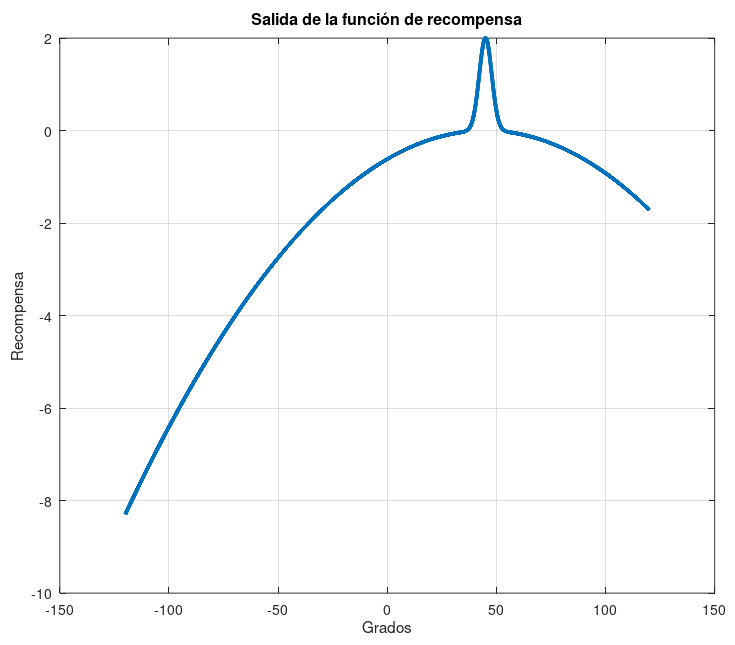
\includegraphics[scale=0.4]{fig/new/Rewardfunc.png}
	\caption{Función de recompensa con $\theta_{objetivo}=45^o$.}
	\label{fig:rewfunc}
\end{figure}

\begin{figure}[hh]
	\centering
	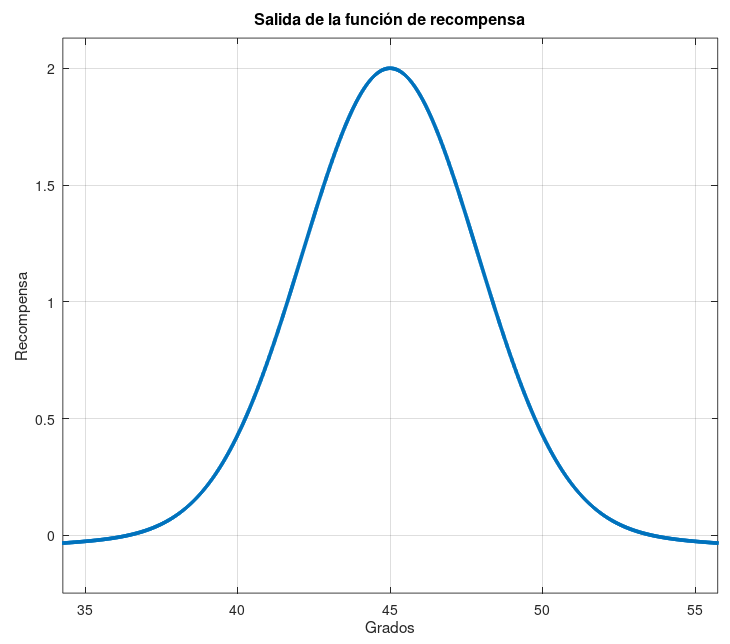
\includegraphics[scale=0.4]{fig/new/Rewardfunccampana.png}
	\caption{$\theta_{correcto}$ con $\theta_{objetivo}=45^o$.}
	\label{fig:rewfunccampana}
\end{figure}
 
Cabe resaltar que para la definición del último punto de la función de recompensas expuesta, se requirió de experimentación con numerosos entrenamientos de los modelos, pues un cambio como la aplicación de una resta lineal
\begin{equation}
R = -C_{\theta} -E_{a_{t-1}} + R_{\theta}
\end{equation}
o prescindir del componente $E_{a_{t-1}}$, da libertad al modelo para explorar sus límites de acción. La aplicación de la técnica de moldear la recompensa (\textit{reward shaping}), impactan sensiblemente el desempeño del agente, en este caso seleccionando la opción del algoritmo \ref{alg:reward} por mantener el nivel del resultado del proceso de entrenamiento estable \cite{RewardShaping}.
 
\subsection{Estructura de las RNA en DQN y PPO}

La estructura general de las RNA en ambos modelos utiliza una capa de entrada definida por el número de observaciones del entorno, anteriormente definido como $obs_n$ en la ecuación (\ref{ecu:observation}), una capa de salida definida por el número de acciones posibles por método, descritos en las siguiente secciones, y un conjunto de tres capas densas (completamente conectadas) con número de neuronas $64$, $128$, $64$, respectivamente, para requerir un aumento de dimensión y acceso a procesamientos más complejos en la RNA, esto definido para cada método \cite{DataScience}.

Como capas de activación, se utiliza ReLU (\textit{rectified linear unit}) por la condición del espacio de acciones base del entorno: valores de PWM en el rango de $0.0$ a $1.0$, de manera que los valores positivos sean recibidos de manera lineal y los negativos ignorados \cite{DataScience}.
 
 
\subsection{DQN}

\subsubsection{Discretización}

Como se mencionó en el capítulo \ref{ch:teoria}, el método DQN se utiliza en el control de sistemas; sin embargo, la literatura indica que DQN tiene problemas en el caso de entornos con espacios de acciones continuos \cite{ForoDQN}.

Por lo tanto, se discretizan las acciones del entorno, que oficialmente trabaja en el rango de $0.0$ a $1.0$ de PWM. De acuerdo con \cite{JorgeBrenes}, el límite superior del espacio de acciones se fija por seguridad en $0.25$ de PWM para cuidar la integridad del equipo real, por lo que se respetó en las pruebas virtuales, además de que la RNAM no conoce el comportamiento de la planta real fuera de ese rango.

Se selecciona una cantidad de $10$ posibles acciones discretas, producto de la experimentación, lo cual responde a la función:
\begin{equation}
a_d = \left\lfloor 36 \cdot a \right\rfloor
\end{equation}
para el proceso de discretización y la función:
\begin{equation}
a = \frac{a_d}{36}
\end{equation}
para el proceso de desdiscretización. Esto deja un espacio de acciones discretas mostradas en la tabla \ref{tab:accionesdis}.
\begin{table}[h]
\centering
\caption{Equivalencia de valores continuos y discretos seleccionados para el método DQN.}
\label{tab:accionesdis}
\begin{tabular}{|l|cccccccccc|}
\hline
\textbf{Tipo}         & \multicolumn{10}{c|}{\textbf{Acción equivalente}}                                                                                                                                                                                                               \\ \hline
Continua (aproximada) & \multicolumn{1}{c|}{0.0} & \multicolumn{1}{c|}{0.03} & \multicolumn{1}{c|}{0.06} & \multicolumn{1}{c|}{0.08} & \multicolumn{1}{c|}{0.11} & \multicolumn{1}{c|}{0.14} & \multicolumn{1}{c|}{0.17} & \multicolumn{1}{c|}{0.19} & \multicolumn{1}{c|}{0.22} & 0.25 \\ \hline
Discreta              & \multicolumn{1}{c|}{0}   & \multicolumn{1}{c|}{1}    & \multicolumn{1}{c|}{2}    & \multicolumn{1}{c|}{3}    & \multicolumn{1}{c|}{4}    & \multicolumn{1}{c|}{5}    & \multicolumn{1}{c|}{6}    & \multicolumn{1}{c|}{7}    & \multicolumn{1}{c|}{8}    & 9    \\ \hline
\end{tabular}
\end{table}

\subsubsection{RNA para DQN}

Tomando la base ya expuesta, la RNA utilizada para el método DQN parte de las estructuras encontradas en repositorios como \cite{PytorchDQN}, utilizando $128$ neuronas en la capa densa central, a la que se le suman una capa densa previa y una capa densa posterior, ambas de $64$ neuronas para el aumento y disminución de la dimensionalidad. Por último, se acopla la capa de salida con las $10$ posibles salidas de valores Q mencionadas. El resultado como tal se muestra en la figura \ref{fig:RNAparaDQN}, de manera que se obtiene un vector $Q_n$ con los valores Q para cada posible acción.

\begin{figure}[hh]
	\centering
	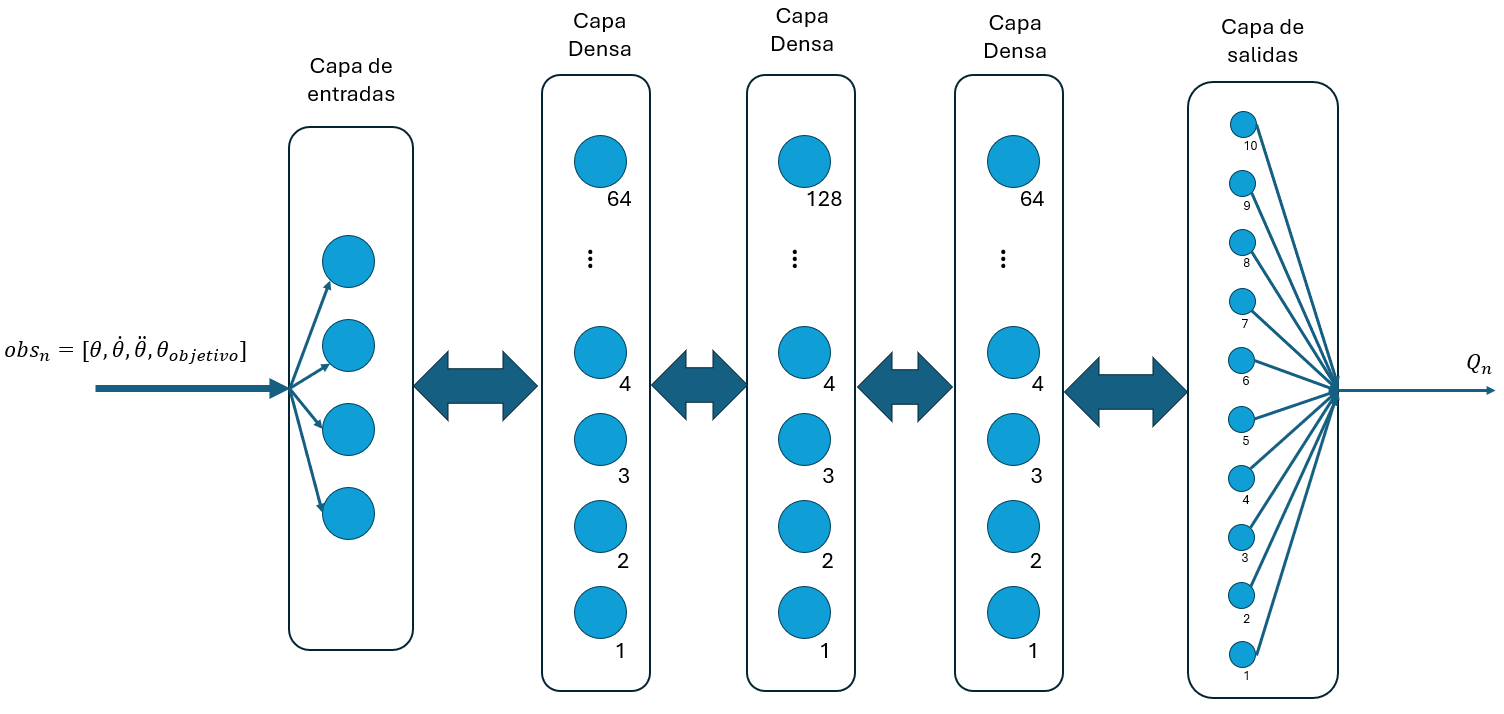
\includegraphics[scale=0.38]{fig/new/RNADQN.png}
	\caption{Estructura de la RNA utilizada en el método DQN.}
	\label{fig:RNAparaDQN}
\end{figure}

\subsubsection{Plan de entrenamiento}

El esquema original de entrenamiento de DQN se modifica en la selección de la acción; utilizando avaro-$\varepsilon$, la etapa de exploración implica la generación de un valor de ruido $n_{ruido}$ que es sumado a la acción discreta dictada por la RNA que aproxima (\ref{ecu:accionDQN}), obteniendo:
\begin{equation}
a_{t_{ruido}} = a_t + n_{ruido}
\end{equation}
donde $n_{ruido}$ varía en principio en un rango con magnitud máxima de $6$ y mínima $0$. Luego al alcanzar la mitad del tiempo de entrenamiento, la magnitud máxima del ruido se reduce a $4$ y luego de tres cuartos del tiempo se reduce a $2$. Por lo tanto, el avaro-$\varepsilon$ reduce las probabilidades de adición de ruido y al mismo tiempo la magnitud del ruido $n_{ruido}$ se diminuye con el avance del entrenamiento, pasando a un método de explotación de lo aprendido.

\subsection{PPO}

\subsubsection{RNA para PPO}

El caso del método PPO cuenta con la misma base de RNA mencionada anteriormente en suma a lo encontrado en los repositorios que implementan el método como \cite{PPOcoding}. Se incorporan tres capas densas compuestas por $64$, $128$ y $64$ neuronas respectivamente, a lo que se suma la capa de salida a una neurona única para el valor de PWM a utilizar. El resultado como tal se muestra en la figura \ref{fig:RNAparaPPO}.

\begin{figure}[hh]
	\centering
	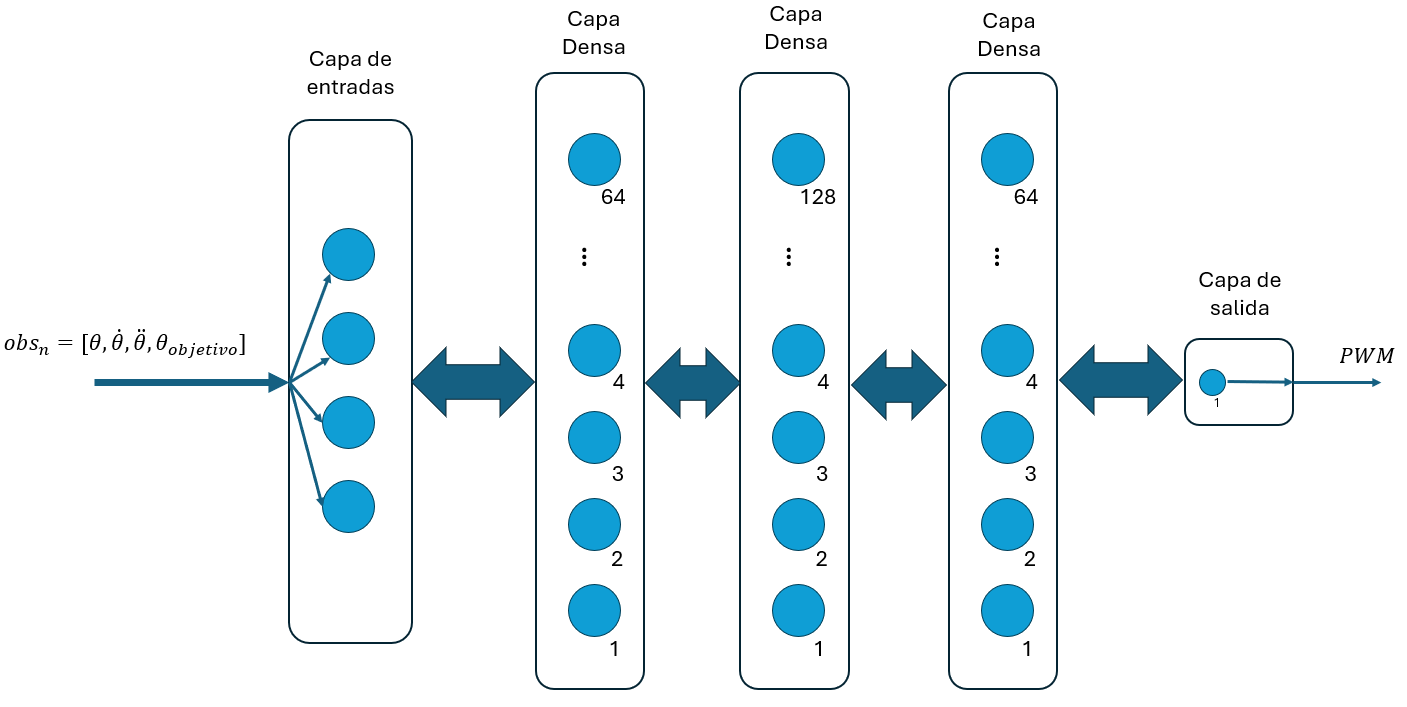
\includegraphics[scale=0.4]{fig/new/RNAPPO.png}
	\caption{Estructura de la RNA utilizada en el método PPO.}
	\label{fig:RNAparaPPO}
\end{figure}


\subsubsection{Plan de entrenamiento}

El algoritmo PPO base define su etapa de exploración con acciones aleatorias muestreadas a partir de una función de distribución normal centrada en la acción tomada por la RNA. En este caso se modificó el procedimiento para cumplir con las siguientes rutinas; se define una muestra de ruido de la distribución pero se fija su uso en una cantidad determinada de iteraciones, en un principio $10$, para ir diminuyendo una unidad cada doceava parte del tiempo de entrenamiento total, esto hasta mantener una muestra por iteración hacia el final del entrenamiento. Este cambio fue necesario para que el ruido agregado le permita al péndulo reaccionar, pues de otro modo la inercia del modelo elimina todo efecto de dicho ruido, que pretende forzar cierta exploración del espacio de estados.

Otra modificación propuesta es la disminución del valor de varianza inicial utilizado, $\sigma^2 = 0.01$ para crear la distribución normal que se muestrea en el punto anterior. La varianza disminuye con el mismo paso que la muestra estática mencionada, pero con una magnitud de $0.001$, esto hasta llegar a un valor mínimo del  $\sigma^2 = 0.001$.

Por último, en lugar de utilizar la muestra directa de la distribución como acción $a_t$, se considera como una muestra de ruido $n_t$ sumada con la señal $a_t$ de la RNA, de la siguiente manera:
\begin{equation}
a_{n} = a_t + n_t
\end{equation}
resultado al que se le limíta la respuesta respetando los valores de seguridad mencionados ($min=0$, $max=0.25$). Al resultado limitado $a'_{n}$ se le sustrae el $a_t$ y se le calcula la probabilidad de aparición del ruido $n'_t$ en la  distribución normal.

Todo los pasos anteriores ocurren durante las pruebas de observación al entorno y respuesta de la RNA, únicamente cambiando sus valores al cumplir el paso de una doceava parte del entrenamiento a la vez.


\subsection{Procesamiento y recopilación de datos}

En el presente proyecto se experimenta con los procesos de entrenamiento de modelos de RL para el control de la planta simulada PAMH, proceso que según se vió en la tabla \ref{tab:MatrizPugh}, requiere recursos computacionales considerables. Los entrenamientos y pruebas se realizaron en un computador con procesador Intel $i7-7700HQ$ de $2.80\, GHz$ con $8$ núcleos, con acceso a una unidad GPU de NVIDIA GeForce GTX $1050$ con $4\, GB$ de VRAM y mediante la herramienta \textit{Google Colab} de la empresa Google, utilizando \textit{Python 3 Google Compute Engine backend} con hasta $12\, GB$ de RAM y $108\, GB$ de almacenamiento.

Por otro lado, el protocolo de todos los procesos de entrenamiento realizados se concentran en la plataforma en línea \textit{Weights $\&$ Biases} (W$\&$B), servicio en línea orientado al aprendizaje automático.



\section{Evaluación de los modelos}

La evaluación del desempeño de los modelos se realiza con el promedio de la recompensa obtenida con el transcurso de los episodios en el entrenamiento de los modelos, donde se comparan diferentes resultados del promedio de la recompensa (diferentes entrenamientos) y se interpretan las aproximaciones a los valores más altos.

Luego de entrenado el modelo, se vuelve a montar el entorno con interfaz Gymnasium y se renderiza el comportamiento del PAMH en su versión virtual. En su segundo episodio se generan una curva de la respuesta angular del entorno respecto al tiempo, tomado directamente del sistema computacional. Con la curva de $\theta$ contra el tiempo en nanosegundos, se calcula el tiempo de subida, el tiempo de asentamiento y el sobreimpulso en la respuesta, esto procurando que el valor final del ángulo se encuentre en un rango de $\pm \, 10\%$ con diferencia al valor deseado $\theta_{objetivo}$.



  \chapter{Resultados y análisis}

En este capítulo se exponen los diseños experimentales realizados para
comprobar el funcionamiento correcto del sistema. Por ejemplo, si se
realiza algún sistema con reconocimiento de patrones, usualmente esta
sección involucra las llamadas \emph{matrices de confusión} donde se
compactan las estadísticas de reconocimiento alcanzadas. En circuitos
de hardware, experimentos para determinar variaciones contra ruido,
etc. También pueden ilustrarse algunos resultados concretos como
ejemplo del funcionamiento de los algoritmos. Puede mostrar por medio
de experimentos ventajas, desventajas, desempeño de su algoritmo, o
comparaciones con otros algoritmos.

Recuerde que debe minimizar los ``saltos'' que el lector deba hacer en
su documento. Por tanto, usualmente el análisis se coloca junto a
\tablas y figuras presentadas, y debe tener un orden de tal modo que se
observe cómo los objetivos específicos y el objetivo general del
proyecto de tesis se han cumplido.

  \chapter{Conclusiones}

Las conclusiones no son un resumen de lo realizado sino a lo que ha llevado el
desarrollo de la tesis, no perdiendo de vista los objetivos planteados desde
el principio y los resultados obtenidos.  En otras palabras, qué se concluye o
a qué se ha llegado después de realizado la tesis de maestría.  Un error
común es ``concluir'' aspectos que no se desarrollaron en la tesis, como
observaciones o afirmaciones derivadas de la teoría directamente.  Esto último
debe evitarse.

Es fundamental en este capítulo hacer énfasis y puntualizar los
aportes específicos del trabajo.

Es usual concluir con lo que queda por hacer, o sugerencias para mejorar los
resultados.



  %----------------------------------------------------------------------------
  % literature in bibtex way:
  % \bibliographystyle{sty/plainurl} % for english documents
  % \bibliography{literatura}
  % literature in biblatex/biber way
  \printbibliography[title={Bibliografía},heading=bibintoc]
  %----------------------------------------------------------------------------

  %----------------------------------------------------------------------------
  \appendix
  %----------------------------------------------------------------------------

  \chapter{Demostración del teorema de Nyquist}
\label{apx:apendice}

El título anterior es solo un ejemplo ilustrativo.  Éste teorema no ameritaría
un apéndice pues es parte normal del currículum de Electrónica, pero apéndices
usualmente involucran aspectos de esta índole, que se salen de la línea de la
tesis, pero que es conveniente incluir por completitud.

Los anexos contienen toda información adicional que se considere pertinente
agregar, como manuales de usuario, demostraciones matemáticas que se salen de
la línea principal de la tesis, pero que pueden considerarse parte de los
resultados del trabajo.


  %----------------------------------------------------------------------------
  \backmatter
  %----------------------------------------------------------------------------

  \printindex                % insert index into document. Don't forget to call
                             % "makeindex filename" first.
\end{document}
